\documentclass[titlepage,10pt,a4paper]{jsbook}

\usepackage{textcomp}

\setcounter{tocdepth}{3}

\usepackage[round,colon,authoryear]{natbib}

\usepackage[dvipdfmx, hiresbb]{graphicx, xcolor}

\usepackage{grffile}

\usepackage[%
dvipdfm,%
pdfstartview={FitH -32768},%    描画領域の幅に合わせる
bookmarks=true,%                しおり付き
bookmarksnumbered=false,%        章や節の番号をふる
bookmarkstype=toc,%             目次情報のファイル.tocを参照
colorlinks=true,%              ハイパーリンクを色文字に
linkcolor=black,%       link の枠の色 black
citecolor=black,%       cite の枠の色 black
urlcolor=black,%        url の枠の色 black
pdftitle={生態学のためのメタバーコーディングとDNAバーコーディング:採集・分子実験編},%
pdfauthor={田辺晶史},
pdfkeywords={メタゲノム, 環境DNA}%
]{hyperref}
\usepackage{pxjahyper}

\usepackage{pxfonts}

\bibliographystyle{jecon}

\makeatletter
\def\maketitle{%
  \begin{center}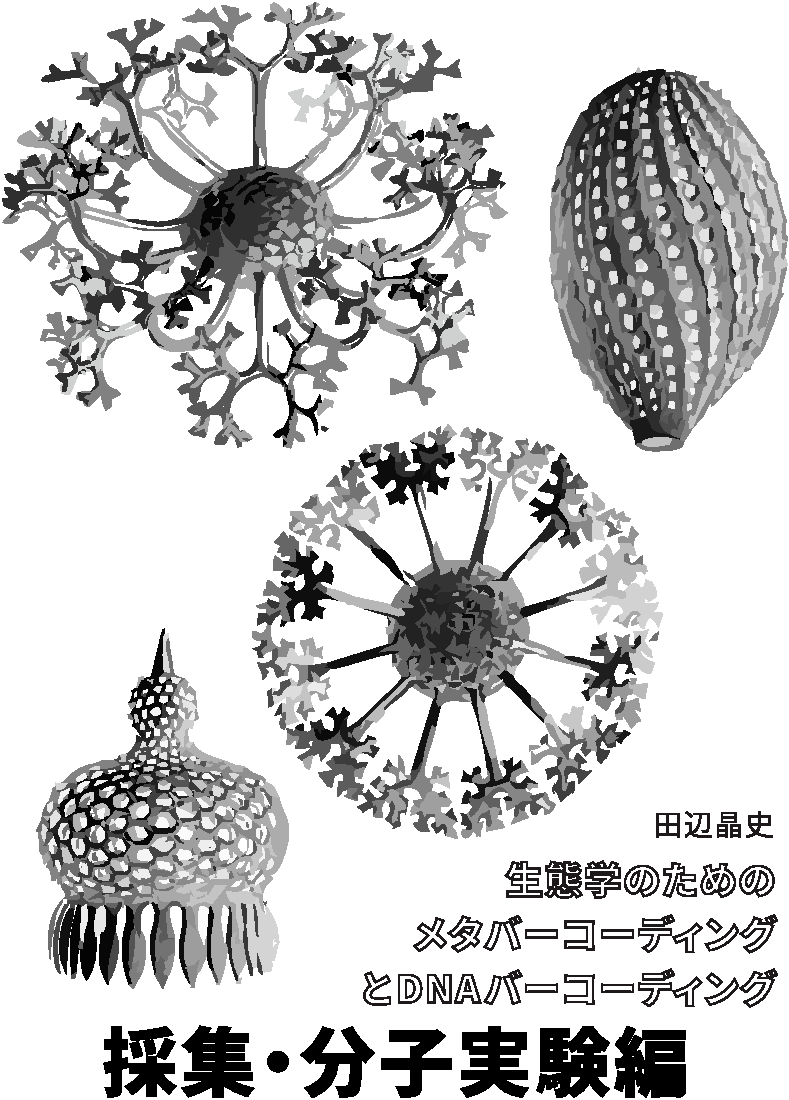
\includegraphics[pagebox=cropbox,clip]{metabarcodingtextbook1.ja.title.pdf}\end{center}%
  \cleardoublepage
  \begin{titlepage}%
    \let\footnotesize\small
    \let\footnoterule\relax
    \let\footnote\thanks
    \null\vfil
    \vskip 60\p@
    \begin{center}%
      {\LARGE \@title \par}%
      \vskip 3em%
      {\large
        \lineskip .75em
        \begin{tabular}[t]{c}%
          \@author
        \end{tabular}\par}%
      \vskip 1.5em
      {\large \@date \par}%
    \end{center}%
    \par
    \@thanks\vfil\null
  \end{titlepage}%
  \setcounter{footnote}{0}%
  \global\let\thanks\relax
  \global\let\maketitle\relax
  \global\let\@thanks\@empty
  \global\let\@author\@empty
  \global\let\@date\@empty
  \global\let\@title\@empty
  \global\let\title\relax
  \global\let\author\relax
  \global\let\date\relax
  \global\let\and\relax
}
\makeatother

\title{生態学のためのメタバーコーディングとDNAバーコーディング:採集・分子実験編}
\author{田辺晶史}
\date{\today}

%\renewcommand{\baselinestretch}{1.2}
\renewcommand{\prepartname}{第}
\renewcommand{\postpartname}{部}
\renewcommand{\prechaptername}{第}
\renewcommand{\postchaptername}{章}
\renewcommand{\presectionname}{}%  第
\renewcommand{\postsectionname}{}% 節
\renewcommand{\contentsname}{目次}
\renewcommand{\listfigurename}{図目次}
\renewcommand{\listtablename}{表目次}
\renewcommand{\refname}{引用文献}
\renewcommand{\bibname}{引用文献}
\renewcommand{\indexname}{索引}
\renewcommand{\figurename}{図}
\renewcommand{\tablename}{表}
\renewcommand{\appendixname}{付録}

\usepackage{float}
\usepackage{framed}
\definecolor{shadecolor}{gray}{0.9}
\newenvironment{content}{\begin{shaded}\vspace{-1em}\raggedright\ttfamily\footnotesize\setlength{\baselineskip}{1.4em}}{\end{shaded}\vspace{-1em}}
\newenvironment{pre}{\begin{leftbar}\raggedright\ttfamily\footnotesize\setlength{\baselineskip}{1.4em}}{\end{leftbar}\vspace{-1em}}
\newenvironment{cmd}{\begin{oframed}\raggedright\ttfamily\footnotesize\setlength{\baselineskip}{1.4em}}{\end{oframed}\vspace{-1em}}

\setlength{\textwidth}{\fullwidth}
\setlength{\evensidemargin}{\oddsidemargin}
\addtolength{\evensidemargin}{-2.5 true mm}
\addtolength{\oddsidemargin}{2.5 true mm}

\makeatletter
\renewcommand{\chapter}{%
  \if@openright\cleardoublepage\else\clearpage\fi
  \global\@topnum\z@
  \secdef\@chapter\@schapter}
\makeatother

\begin{document}
\thispagestyle{empty}
\maketitle
\cleardoublepage
\pagenumbering{roman}
\tableofcontents
\cleardoublepage
\setlength{\parindent}{0em}
\setlength{\parskip}{1em plus 0.2em}
\parindent=0em
\parskip=1em plus 0.2em
\pagenumbering{arabic}

\chapter*{はじめに}
\addcontentsline{toc}{chapter}{はじめに}

本書はクリエイティブ・コモンズの表示-継承 4.0 国際ライセンスの下で配布します。
このライセンスの下では、原著作者の明示を行う限り、利用者は自由に本書を複製・頒布・展示することができます。
また、原著作者の明示と本ライセンスまたは互換性のあるライセンスの適用を行う限り、本書を改変した二次著作物の作成・配布も自由に行うことができます。
詳しい使用許諾条件を見るには\\
\href{https://creativecommons.org/licenses/by-sa/4.0/}{https://creativecommons.org/licenses/by-sa/4.0/}\\
をチェックするか、クリエイティブ・コモンズに郵便にてお問い合わせください。
住所は Creative Commons, PO Box 1866, Mountain View, CA 94042, USA です。

本書が皆さんの役に立つことができましたら幸いです。
この機会を与えて下さった京都大学生態学研究センターの東樹宏和博士、水産研究・教育機構中央水産研究所の長井敏博士、龍谷大学の山中裕樹博士と、本書をお読みの皆さんに感謝します。

\chapter{環境DNA・メタゲノムDNAの採集方法}

ここでは、水からの環境DNA採集、および水、土壌、糞などからのメタゲノムDNAの採集方法について解説します。
DNA抽出用の個体や組織の採集方法はここでは取り扱いません。
なお、環境DNAとメタゲノムDNAは識別困難ですが、ここでは、環境DNAを「生物個体から排出されたDNA」、メタゲノムDNAを「生物個体から排出されていないDNA」ということにします。
したがって、水中の魚類や甲殻類、水生昆虫、水生植物のDNAは環境DNAであり、微生物のDNAはメタゲノムDNAであることが多いでしょう(ただし、区別できないだけで微生物の環境DNAも含まれているでしょう)。
また、未消化物に含まれる被食者や本人のDNAはどちらにするか難しいところですが、とりあえずメタゲノムDNAということにしておきます。

\section{サンプリングデザイン}

採集地点・時間をどのように配置するかは研究の内容に直結する重要な課題です。
ここで研究目的の達成の可否が決まると言っても過言ではありません。
そのためには、研究目的の明確化と予備調査が必須です。

例えば、ため池ごとの魚類相と環境条件(池の大きさ、深さ、水質、地質、高度、緯度経度など)との関連性を解明したいが、ため池の中での微細な違いには興味がないケースでは、ため池がよほど小さくない限り、ため池内の数地点から水を採集し、混合して濾過採集することになります。
ため池が非常に小さい場合や、ため池内の水が十分に混合されていたり、対象となるため池があまりに多い場合は、1地点だけでため池を代表させることもあるでしょう。
もちろん、余裕があるならため池内の数地点のサンプルを全て別々にして、その気になればため池内の微細な違いをも解析可能にしておくことも悪くありませんが、後述するサンプルレプリケートを複数用意することを考えると、大きな労力が必要となりますので、人手を十分考慮する必要があります。
また、その場合はため池内の数地点のサンプル間でDNA抽出効率・PCR増幅効率などに大きな違いが生じることがないようにしなくてはなりません(違う場合は環境条件の影響と言えなくなってしまう)。

別のケースとして、森林の土壌を分析して、微生物叢と植物相の関連性を解明したい場合を考えましょう。
この場合、1地点を広くかつ深く取り、その範囲の土壌を混合して採集するか、その範囲の土壌からいくつかのサブサンプルを採集して混合するのがよいでしょう。
土壌では、少し離れただけで全く異なる微生物叢を示すので、ある場の植物相と対応する微生物叢を完全な1点では代表することができません。
そのため、植物相と対応する範囲の数地点のサブサンプルをプールすることで代表させます。

以上のように、「DNAの拡散する範囲」と「そのサンプルで代表させたい範囲」を考慮して、前者の範囲の方が広くなるようにサンプリングデザインを行う必要があります。
後者の範囲の方が広くなってしまう場合、研究の目的とする議論が行えなくなることがあります。
ただ、後者の範囲の方が広くなる場合でも、サンプルが大量にあるのであれば、「本来の生物相」と「サンプルの生物相」との乖離に何らかの偏りがない限りは目的の議論ができる場合もあるでしょう。

また、濾過採集を行う場合、濾過水量も結果に大きな影響を及ぼすことが知られています。
ただ、無制限に濾過水量を増やすことは不可能なため、現実的に実施可能な範囲で最大の水量を濾過するようにしている例が多いようです。

\section{テクニカルレプリケートとネガティブコントロール}

1サンプルを1レプリケートで採集した場合、DNA抽出効率やPCR増幅効率のばらつきの影響を受けます。
また、レアな種のゲノムDNAや低濃度の環境DNAはサンプルに入ったり入らなかったりすることもあり得ます。
そこで、可能であれば複数(3以上ならなお良い)のレプリケートを1サンプル中に用意することが望ましくなります。
このようにすることで、各サンプルごとに種の「発見率」を推定することができます。
例えば、1サンプルが10レプリケート含んでいるとき、x軸をレプリケート数、y軸を合計種数とする折れ線グラフを描くことを想像してください。
10レプリケートからx軸のレプリケート数だけ無作為抽出して合計種数を算出してy軸の合計種数を計算します。
このとき、折れ線が傾きゼロの直線なら1レプリケートでも発見率は100\%と考えられ、x=1では傾きゼロではなくとも、x=10では傾きゼロになっているなら10レプリケート合計すれば飽和している=発見率100\%ということになります。
しかし、x=10でも線が傾いているようであれば、発見率は100\%ではなく、いくらか取りこぼしがあることがわかります。
発見率が100\%であることが理想ですが、必ずしもそうである必要はありません。
重要なのは、発見率が推定できることです。

\section{水からの濾過採集方法}

\subsection{濾過フィルターの選定}

メタゲノム・環境DNA採集に適した濾過フィルターには、形状・材質・粒子保持能で分けると以下の種類があります。ディスクフィルターはひとまず47mmのものを挙げておきますが、より小さいものや大きいものもあります。

\begin{itemize}
\item カートリッジ型フィルター
\begin{itemize}
\item PVDF製濾過膜
\begin{itemize}
\item 0.45{\textmu}m Millipore Sterivex-HV SVHV010RS
\item 0.22{\textmu}m Millipore Sterivex-GV SVGV010RS
\end{itemize}
\item PES製濾過膜
\begin{itemize}
\item 0.22{\textmu}m Millipore Sterivex-GP SVGP01050
\end{itemize}
\end{itemize}
\item 47mmディスクフィルター
\begin{itemize}
\item グラスファイバー製濾紙
\begin{itemize}
\item 1.2{\textmu}m Whatman GF/C 1822-047
\item 0.7{\textmu}m Whatman GF/F 1825-047
\item 0.7{\textmu}m Millipore AP40 AP4004705
\end{itemize}
\item ポリカーボネート製濾過膜
\begin{itemize}
\item 12.0{\textmu}m Whatman Nuclepore 111116
\item 10.0{\textmu}m Whatman Nuclepore 111115
\item 10.0{\textmu}m Millipore Isopore TCTP04700
\item 8.0{\textmu}m Millipore Isopore TETP04700
\item 5.0{\textmu}m Millipore Isopore TMTP04700
\item 3.0{\textmu}m Whatman Nuclepore 111112
\item 3.0{\textmu}m Millipore Isopore TSTP04700
\item 2.0{\textmu}m Whatman Nuclepore 111111
\item 2.0{\textmu}m Millipore Isopore TTTP04700
\item 1.2{\textmu}m Millipore Isopore RTTP04700
\item 1.0{\textmu}m Whatman Nuclepore 111110
\item 0.8{\textmu}m Millipore Isopore ATTP04700
\item 0.6{\textmu}m Millipore Isopore DTTP04700
\item 0.4{\textmu}m Millipore Isopore HTTP04700
\item 0.22{\textmu}m Millipore Isopore GTTP04700
\end{itemize}
\item セルロース混合エステル製濾過膜
\begin{itemize}
\item 8.0{\textmu}m Millipore MF-Millipore SCWP04700
\item 5.0{\textmu}m Millipore MF-Millipore SMWP04700
\item 3.0{\textmu}m Millipore MF-Millipore SSWP04700
\item 1.2{\textmu}m Millipore MF-Millipore RAWP04700
\item 0.8{\textmu}m Millipore MF-Millipore AAWP04700
\item 0.65{\textmu}m Millipore MF-Millipore DAWP04700
\item 0.45{\textmu}m Millipore MF-Millipore HAWP04700
\item 0.3{\textmu}m Millipore MF-Millipore PHWP04700
\item 0.22{\textmu}m Millipore MF-Millipore GSWP04700
\end{itemize}
\item PVDF製濾過膜
\begin{itemize}
\item 0.45{\textmu}m Millipore Durapore HVLP04700
\item 0.22{\textmu}m Millipore Durapore GVWP04700
\end{itemize}
\item PES製濾過膜
\begin{itemize}
\item 0.45{\textmu}m Millipore Millipore Express PLUS HPWP04700
\item 0.22{\textmu}m Millipore Millipore Express PLUS GPWP04700
\end{itemize}
\end{itemize}
\end{itemize}

カートリッジ型の方が事前に塩素漂白しないといけないものが少なく準備が楽で、コンタミネーションはしにくいと考えられます。
ただし高価で濾過膜の選択肢が少ないというデメリットがあります。
ディスクフィルターは事前に塩素漂白しないといけないものが多いため準備の手間が多く、コンタミネーションしやすいですが、その代わり安価で濾過膜の選択肢が多くあります。

ポリカーボネート製濾過膜は孔径が極めて均一で粒子サイズごとの分画に適し、様々な孔径の品が揃えられています。
デメリットとしては、空隙率が低く濾過が遅い、目詰まりしやすい、そして高価という点があります。
セルロース混合エステルは孔径はポリカーボネートほど均一ではありませんが、孔径の選択肢は多く、空隙率が非常に高いため濾過が早い上、ポリカーボネートに比べれば安価です。
ポリエーテルスルホン(PES)とポリフッ化ビニリデン(PVDF)も空隙率が高く濾過はポリカーボネートよりずっと早くなります。
グラスファイバーもポリカーボネートに比べて空隙率が高く濾過はずっと早いですが、孔径の均一性は最も低く、その上DNA・RNAを吸着しやすい性質があります(DNA・RNAの抽出にも利用されるくらいです)。
しかし、グラスファイバーが最も安価です。

また、濾過フィルターの選択はDNAの抽出方法にも影響を及ぼします。
カートリッジ型の場合、バッファーを注入してインキュベートすることでバッファー中にDNAを溶解させ、逆さまにして遠心することで回収します\citep{Miya2016}。
微生物メタゲノムの場合、ジルコニアビーズなどをカートリッジ内に入れて破砕処理を加えることで抽出効率を改善することもできます\citep{Ushio2019}。
ディスクフィルターからの環境DNAの回収では、最初にフィルターを筒状に丸めてザリベットや空カラム(吸着剤の入っていないスピンカラム)に入れ、そこにバッファーを加えてインキュベートすることでDNAを溶解します。
ディスクフィルターから微生物メタゲノムを回収する場合、バッファー中でフィルターを切り刻んでジルコニアビーズを加えて破砕処理を行います。
このため、グラスファイバー製などの剪刀で刻みにくいフィルターは使用できません。

\subsection{濾過方法の選定}

濾過の方法には、以下の4通りがあります。

\begin{enumerate}
\item シリンジを用いて手動で加圧する
\item 真空ポンプを手動で動かして吸引する
\item ペリスタルティックポンプなどを電気で動かして加圧する
\item 真空ポンプを電気で動かして吸引する
\end{enumerate}

どの方法を用いても構いませんが、電気が使えない場所では1を、電気が使える場所では4を使うのが主になると思います。
採水後にすぐには濾過できない場合、10\%塩化ベンザルコニウム溶液(オスバンSという名前で薬局で販売されている)を1L当たり1mL加える(終濃度0.01\%)ことで、細菌による環境DNAの分解を抑制できるという報告\citep{Yamanaka2017}があり、近年よく利用されているようです。

\subsection{サンプル固定方法の選定}

濾過サンプルの固定方法は、主に以下の方法が考えられます。

\begin{enumerate}
\item 可能な限り水抜きしてDNA・RNA固定液(作成法は付録\ref{makingRNAlater}を参照)を加える
\item 可能な限り水抜きしてTEバッファーを加える
\item 可能な限り水抜きしてエタノールを加える
\item 可能な限り水抜きして冷凍する
\end{enumerate}

最近の論文を読む限りでは、1と4がよく使われているようです。4以外は冷蔵、あるいは常温保管することも可能です。

\subsection{濾過関連機材の塩素漂白の方法}

\subsubsection{必要な機材}
\begin{itemize}
\item 水道
\item 蛇口に適合するシリコンチューブ (厚さは任意): 1本
\item 漂白剤抜き器 (作成方法は付録\ref{makingdebleachcontainer}を参照): 1個
\item 漂白対象物が入る大きさの容器: 1個
\item 防水エプロン: 1着
\item ショーワグローブ No.140 腕カバー付厚手: 1双
\end{itemize}

\subsubsection{必要な消耗品}
\begin{itemize}
\item 花王 ハイターE (界面活性剤なしの塩素系漂白剤。次亜塩素酸ナトリウム6\%): 適量
\item SPW: 適量
\end{itemize}

\subsubsection{作業手順}
\begin{enumerate}
\item 漂白対象物が入る大きさの容器に漂白対象物を入れる
\item 漂白対象物が浸かるように水道水を注ぐ
\item 水道水の5--10\%量のハイターEを入れてかき混ぜる
\item 漂白対象物が水に浮く場合、同サイズの容器を重ねて重しを入れて押さえつける (これができるような形状の容器を使用する)
\item 時々ゆすりながら10分以上、できれば1時間以上浸ける (ただし浸け過ぎに注意)
\item 漂白液を捨てて漂白対象物を漂白剤抜き器に移す
\item 漂白剤抜き器のホースニップルと水道の蛇口をシリコンチューブで接続する
\item 水道水を上限まで注いで捨てる
\item 漂白対象物が
\begin{enumerate}
\item 水に浮く場合、水道水を勢いよく流しっぱなしにして30分以上放置して水を捨てる (水の勢いで漂白対象物が動くようにする)
\item 水に沈む場合、水道水を上限まで注いで捨てることを更に2回繰り返す
\end{enumerate}
\item 漂白対象物が入る大きさの容器に漂白対象物を移す
\item SPWを漂白対象物が浸かるように注いですすいで捨てる
\item 乾燥が必要な場合はアルミホイルに包んで常温--60℃で乾燥する (60℃にする前に一度200℃以上で庫内を滅菌してから60℃に下げること)
\end{enumerate}

なお、漂白剤抜き器を漂白対象物が入る大きさの容器として使用しても問題ありません。
また、全ての作業を同じ容器(漂白剤抜き器を含む)で行っても構いません。
フィルターホルダーはパッキンやアダプタを外して分解し、個別に漂白を行い、漂白後に組み立てます。

\subsection{吸引濾過装置を用いた水からの微生物メタゲノムDNA・環境DNAの濾過採集方法}

\subsubsection{必要な機材}
\begin{itemize}
\item DC12Vのシガーソケット搭載車 または ACアダプタ: 1個
\item 車載用吸引ポンプユニット (作成方法は付録\ref{makingpumpunit}を参照): 1個
\item 吸引濾過装置 (作成方法は付録\ref{makingfilteringunit}を参照): 1個
\item toolsisland 手動式オイルチェンジャー または メルテック オイルチェンジャー OC-060: 1個
\item アズワン 穴付きシリコン栓 8号 (1-7650-01) の両方の穴に 光 ステンレス丸パイプ 外径6mm を適当な長さに切断して挿したもの (長さを不揃いにすること): 1個
\item アズワン シリコンチューブ 内径5mm 外径11mm 長さ1m (6-586-19-01): 1本
\item アズワン シリコンチューブ 内径5mm 外径11mm 長さ1m (6-586-19-01) を切断して途中に Whatman VACU-GUARD (6722-5000) を挟んだもの: 1本
\item モンキーレンチ: 1本 (ディスクフィルター使用時のみ)
\item サンダイヤ デッキ型ピンセット 125mm (アズワン品番 6-531-12): 1本 (ディスクフィルター使用時のみ)
\item ハサミ: 1本
\item ライター: 1本
\item ゼブラ マッキープロ細字 特殊用途DX: 1本 (色の薄いハズレ個体がよくあるので予め確認しておく)
\item 三菱アルミニウム 三菱ホイル タフ 30cm x 50m: 1本
\item ロゴス ハイパー氷点下クーラーM No.81670070: 1個
\item ロゴス 倍速凍結・氷点下パックXL No.81660640: 2個以上 (必ず氷点下を維持できる保冷剤を使用すること)
\end{itemize}

\subsubsection{必要な消耗品}
\begin{itemize}
\item 以下のいずれかの濾過フィルターユニット: 1個 / 1サンプル
\begin{itemize}
\item アズワン FH-PP47 (3-6736-01) または ADVANTEC PP-47 に47mmディスクフィルターを詰めたもの (漂白で再利用可)
\item Millipore Sterivex-HV 0.45{\textmu}m PVDF SVHV010RS
\item Millipore Sterivex-GV 0.22{\textmu}m PVDF SVGV010RS
\item Millipore Sterivex-GP 0.22{\textmu}m PES SVGP01050
\end{itemize}
\item フィルターユニットに適合するアダプタ (作成方法は付録\ref{makingfilteradapter}を参照): 1個 / 1サンプル (漂白で再利用可)
\item 以下のいずれかのプラスチックバッグ: 1個 / 1サンプル
\begin{itemize}
\item カウパック 夢パック 100mL DP16-TN0100
\item カウパック 夢パック 200mL DP16-TN0200
\item カウパック 夢パック 300mL DP16-TN0300
\item カウパック 夢パック 500mL DP16-TN0500
\item カウパック 夢パック 1000mL DP16-TN1000
\end{itemize}
\item 以下のいずれかの使い捨てビーカー: 1個 / 1サンプル
\begin{itemize}
\item 大塚刷毛製造 補修用カップ 容器のみ 400mL 3221110400
\item 大塚刷毛製造 補修用カップ 容器のみ 600mL 3221110600
\item 大塚刷毛製造 補修用カップ 容器のみ 800mL 3221110800
\item ビッグ 調色ミキシングカップ 1000mL MK11L
\end{itemize}
\item セイニチ ユニパック C-4: 1枚 / 1サンプル
\item 使い捨てポリ手袋: 2双 / 1サンプル
\end{itemize}

\subsubsection{作業手順}
\begin{enumerate}
\item 車載用吸引ポンプユニットのバルブは開放しておく
\item 吸引濾過装置のバルブは全て閉じておく
\item シガーソケットに車載用吸引ポンプユニットの電源を接続する
\item 車載用吸引ポンプユニットのホースニップルにVACU-GUARDを取り付けたシリコンチューブ経由で穴付きシリコン栓の短い方のステンレスパイプを接続する
\item 穴付きシリコン栓を手動式オイルチェンジャーのタンクに挿す
\item 穴付きシリコン栓の長い方のステンレスパイプにもう一つのシリコンチューブ経由で吸引濾過装置を接続する
\item ポリ手袋を着ける
\item 使い捨てビーカーで必要量の水試料を量り取り、プラスチックバッグに入れる
\item 濾過フィルターユニットにアダプタを取り付ける (ディスクフィルター使用の場合はモンキーレンチでしっかり締め付ける)
\item アダプタの反対側に水試料の入ったプラスチックバッグを取り付ける (アダプタの接着面に力がかからないように注意すること)
\item プラスチックバッグ+濾過フィルターユニットを濾過フィルターユニットが下になるように吸引濾過装置に取り付け、リピートバンドを締める
\item 吸引濾過装置のバルブ(プラスチックバッグからタンクの経路上のもの)を開ける
\item 車載用吸引ポンプユニットの電源を入れ、水試料を吸引する
\item 水試料吸引開始後、プラスチックバッグ上端にハサミで切り込みを入れる (ハサミが水試料に接さないように注意。必要に応じてハサミをライターで火炎滅菌する)
\item 水試料の吸引が終わったら、吸引濾過装置の濾過フィルターユニット直下のバルブを閉じる
\item リピートバンドを緩めてプラスチックバッグ+濾過フィルターユニットを吸引濾過装置から外す
\item 濾過フィルターユニットからプラスチックバッグを取り外して捨てる (アダプタは残す)
\item 濾過フィルターユニットを再度吸引濾過装置に取り付け、濾過フィルターユニット直下のバルブを開けて濾過フィルターユニット内の残留水を吸引する (濾過フィルターユニットを独楽のように回して吸引する)
\item アルミホイルを適当な長さで切って折り目を付けておく
\item 吸引濾過装置の濾過フィルターユニット直下のバルブを閉じて車載用吸引ポンプユニットの電源を切る
\item 濾過フィルターユニットを吸引濾過装置から外す
\item ポリ手袋を交換する
\item 濾過フィルターユニットが
\begin{enumerate}
\item フィルターホルダー+ディスクフィルターの場合、アダプタはそのままにして分解し、フィルターを分解してライターで火炎滅菌したピンセットで濾液入力面を内側にして二つ折りにし、アルミホイルで包んでマッキープロでサンプル情報を記述しユニパックに入れ、クーラーバッグに保冷剤で挟まれるように入れる
\item Sterivexの場合、アダプタを外してマッキープロでサンプル情報を記述し、アルミホイルで包んでからユニパックに入れ、クーラーバッグに保冷剤で挟まれるように入れる (ユニパックにもサンプル情報を記述しておく)
\end{enumerate}
\item ポリ手袋を外して捨てる
\item 吸引濾過装置の両側下部バルブを開放する (吸引濾過装置内の残留水がタンクに吸い込まれる)
\item 手動式オイルチェンジャーのタンクからシリコン栓を外し、中の廃液を捨てる
\end{enumerate}

なお、アズワンFH-PP47およびADVANTEC PP-47のパッキンが劣化した場合、シリコンゴムかフッ素ゴム製のAS568-030型およびAS568-033型の品に交換することができます。
ここではSterivexをすぐに冷凍する方法を示しましたが、中にDNA・RNA固定液(作成法は付録\ref{makingRNAlater}を参照)を注入して両端にキャップ(テルモ テルフュージョン三方活栓キャップ密栓用 XX-WS01K* および コクゴ 点眼キャップ赤3φ 101-5210102)を付けて冷凍・冷蔵・常温保管する方法もあります(DNA・RNA固定液を注入しない場合もDNA抽出時にはキャップを使用することになるので、採集時に付けておくのも良いでしょう)。
海外などで冷凍手段が確保できない場合にはこの方法を用いることになります。

\subsection{シリンジを用いた水からのメタゲノムDNA・環境DNAの濾過採集方法}

\subsubsection{必要な機材}
\begin{itemize}
\item タジマ コーキングガン コンボイVS CNV-VS: 1個 (先端の円筒部内側に、ワッシャーがくっつくようコクヨ マク-S340をカットして貼っておく)
\item ゼブラ マッキープロ細字 特殊用途DX: 1本 (色の薄いハズレ個体がよくあるので予め確認しておく)
\item 三菱アルミニウム 三菱ホイル タフ 30cm x 50m: 1本
\item ロゴス ハイパー氷点下クーラーM No.81670070: 1個
\item ロゴス 倍速凍結・氷点下パックXL No.81660640: 2個以上 (必ず氷点下を維持できる保冷剤を使用すること)
\item 大阪魂 丸ワッシャー 特寸 鉄/ユニクロ M21 x 外径50mm x 厚さ3.2mm 4個入 (42175375) または 同 70個入 (41954954): 1枚
\item サンダイヤ デッキ型ピンセット 125mm (アズワン品番 6-531-12): 2本
\item シンワ測定 数取器 台付 75078 または 新潟精機 数取器 台付型 C-4B: 1個
\item ライター: 1個
\end{itemize}

\subsubsection{必要な消耗品}
\begin{itemize}
\item テルモ テルモシリンジ ロック付 50mL SS-50LZ または JMS 注射針なしシリンジ ロックタイプ 50mL JS-S50L: 1本 / 1サンプル
\item 以下のいずれかの濾過フィルターユニット: 1個 / 1サンプル
\begin{itemize}
\item Millipore Sterivex-HV 0.45{\textmu}m PVDF SVHV010RS
\item Millipore Sterivex-GV 0.22{\textmu}m PVDF SVGV010RS
\item Millipore Sterivex-GP 0.22{\textmu}m PES SVGP01050
\end{itemize}
\item 以下のいずれかの使い捨てビーカー: 1個 / 1サンプル
\begin{itemize}
\item 大塚刷毛製造 補修用カップ 容器のみ 400mL 3221110400
\item 大塚刷毛製造 補修用カップ 容器のみ 600mL 3221110600
\item 大塚刷毛製造 補修用カップ 容器のみ 800mL 3221110800
\item ビッグ 調色ミキシングカップ 1000mL MK11L
\end{itemize}
\item セイニチ ユニパック C-4: 1枚 / 1サンプル
\item 使い捨てポリ手袋: 1双 / 1サンプル
\end{itemize}

\subsubsection{作業手順}
\begin{enumerate}
\item ポリ手袋を着ける
\item ピンセット2本を火炎滅菌し、そのピンセットを用いてワッシャーを火炎滅菌し、コーキングガン先端にワッシャーの面が取れている方がSterivexに接するようセットする
\item セットしたワッシャーが何かに触れないようにコーキングガンをどこかに吊り下げる
\item 手を使わずにボタンを押せるように数取器を設置する
\item 使い捨てビーカーで必要量の水試料を量り取る
\item シリンジにビーカーから水試料50mLを吸い取る (水に浸かるシリンジ先端3cm程度は触れないようにする)
\item シリンジのルアーロック部にSterivexを取り付ける
\item コーキングガン先端のワッシャーの穴からSterivexが突き出すようにセットする
\item Sterivexが下になるように垂直に立ててコーキングガンの引き金を引いて加圧濾過する (加圧しすぎると壊れるので、水が出るのを待つこと)
\item 50mLの濾過が終わったら、数取器のボタンを手を使わずに押してカウントアップ
\item シリンジ+Sterivexをコーキングガンから抜いてSterivexとシリンジを分離する
\item 必要量に達するまで6--11を繰り返す (濾過に必要な圧力が大きくなってきたら無理せず複数本に分ける)
\item 必要な水量の濾過が終わったら、シリンジに空気をめいっぱい吸引する
\item シリンジのルアーロック部にSterivexを取り付けてワッシャーに通す
\item Sterivexが先端から突き出すようにコーキングガンにセットする
\item Sterivexが下になるように垂直に立ててコーキングガンの引き金を引き、できるだけSterivex内の水を抜く
\item シリンジ+Sterivexをコーキングガンから抜いてSterivexとシリンジを分離する
\item Sterivexをアルミホイルで包んでから、マッキープロでサンプル情報を記述したユニパックに入れ、クーラーバッグに保冷剤で挟まれるように入れる
\item ポリ手袋を外して捨てる
\end{enumerate}

ワッシャーは、サンプル数分用意して予め乾熱滅菌し、アルミホイルで個包装しておくことで火炎滅菌を省略できます。
JMSのシリンジには100mLタイプ(JS-S00L)もあります。
高価ですが、濾過作業の反復数を半減させることができます。
これを用いる場合、金属製のワッシャーの代わりに、呼び径40の塩ビVP管(内径40mm・外径48mm)を15mmの長さに切断したものを使用します。
塩ビ管は予め塩素漂白してアルミホイルで個包装しておきます。
50mLシリンジとワッシャーの組み合わせでは、ワッシャーからはSterivexだけが突き出る形になりますが、100mLシリンジと塩ビ管の組み合わせでは、Sterivexとシリンジの先端半分以上が塩ビ管から突き出るようにして塩ビ管でフランジを支えます。
ここではSterivexをすぐに冷凍する方法を示しましたが、中にDNA・RNA固定液(作成法は付録\ref{makingRNAlater}を参照)を注入して両端にキャップ(テルモ テルフュージョン三方活栓キャップ密栓用 XX-WS01K* および コクゴ 点眼キャップ赤3φ 101-5210102)を付けて冷凍・冷蔵・常温保管する方法もあります(DNA・RNA固定液を注入しない場合もDNA抽出時にはキャップを使用することになるので、採集時に付けておくのも良いでしょう)。
海外などで冷凍手段が確保できない場合にはこの方法を用いることになります。

\chapter{DNA抽出・ライブラリ調製・シーケンシング}

\section{機材・試薬の滅菌とDNA分解によるコンタミネーションの抑制}

マイクロピペットで使用するチップは全てフィルターチップにします。
ただし、DNAを含む溶液を吸わない場合にはフィルターのないチップを使っても構いません。
例えば、10mLチップでDNAを含む溶液を吸うことは考えにくいので、10mLチップはフィルターなしで問題ないと思います。

使用する機材や試薬は、以下のようにいくつかの方法を用いて滅菌およびDNA分解を行うことでコンタミネーションを抑制します。

\begin{description}
\item[金属製またはフッ素樹脂機材] オーブンを用いて乾熱滅菌する。250℃で30分。
\item[ガラスまたはフェノール樹脂機材] オーブンを用いて乾熱滅菌する。200℃で4時間。
\item[PBT樹脂機材] オーブンを用いて乾熱滅菌する。180℃で8時間。
\item[その他のプラスチック機材] タライで塩素漂白する。20倍希釈漂白液で10分。
\item[乾熱滅菌、塩素漂白できない機材] DNA-OFFを染み込ませたペーパータオルで拭き取る。
\item[試薬] ガラス瓶に入れてオートクレーブして冷まし、クリーンベンチ内で紫外線を照射する。
\end{description}

ただし、当該処理を行うと著しく劣化したり分解する場合は行わないように注意が必要です(例えば、PEG8000を含む溶液をオートクレーブしてはいけません)。
作業後の実験台やマイクロピペットはDNA-OFFを染み込ませたペーパータオルで拭き取ります。
作業後のプラスチック製チューブラックは塩素漂白します。
恒温槽のブロックや金属製のローターは水道水で洗浄してからSPWですすいで乾かします。
インキュベータは250℃まで上げられるものであれば、250℃で30分ほど内部を乾熱滅菌します。

遠心機は、トミー精工のMXシリーズ・MDXシリーズを用いると、樹脂製のローターが使用できるため、塩素漂白が可能です。
トミー精工MDXシリーズ用ローターTAR015-SC18と専用トレーTRA-01を使用すると、スピンカラムの頻繁な差し替えを減らし、廃液を1本ずつ捨てる作業をなくすことができます。
15mL遠沈管やSterivexの遠心には、トミー精工LCX-200にTS-33CスイングロータとB433バケット、3315-TC04Pラックの組み合わせや、久保田商事Model 4000にST-2504MSスイングロータと055-1160ラックの組み合わせ、himac CT6EにT5SSスイングロータとS409814Aラックの組み合わせが便利です。
これらの製品はラックが樹脂製のため、塩素漂白が可能です(ただし、メーカーは推奨していない場合があります)。
スイングロータを使用するのは、Sterivexの中からの排液量・残液量を均一にし、再現性を高めるためです。
DNA抽出・PCR前の準備を行う部屋と、PCRおよびPCR後の操作を行う部屋は分離し、相互に行き来をしない、あるいは行き来をする場合も各部屋専用の白衣、マスク、キャップを使用するなど、PCRによる増幅後のDNAのコンタミネーションに細心の注意を払う必要があります。
DNA抽出では汚れたものも扱うため、DNA抽出とPCR前の準備もできれば別の部屋に分けた方が良いでしょう。
クリーンベンチを活用すれば部屋の数は減らせますが、少なくともPCR前とPCR以降で2部屋は必要です。
筆者の場合、ディスクフィルターからのDNA抽出のためにフィルターを丸めてスピンカラムに入れる作業、PCR前の準備をしてから、鋳型としてのPCR産物を加える作業だけ、クリーンベンチ内で行っています(作業中、ファンは使用しない)。

\section{テクニカルレプリケートとネガティブコントロール}

あとでかく。

\section{DNA抽出}

\subsection{固形サンプル(濾過フィルター以外)からのDNA抽出プロトコル}

必要な試薬の作成方法は付録\ref{makingDNAextractionbuffers}を参照してください。

\subsubsection{必要な機材}
\begin{itemize}
\item 恒温槽またはインキュベータ: 1台
\item 1.5/2mLチューブ20000×g対応遠心機: 1台
\item HOZAN ピンセット P-888: 1本
\item ライター: 1本
\item 100{\textmu}Lチップ用マイクロピペット: 1本
\item 200{\textmu}Lチップ用マイクロピペット: 1本
\item 1000{\textmu}Lチップ対応マイクロピペット: 1本
\item エー・アンド・デイ 10mLチップ対応電動ピペット MPA-10000: 1本
\end{itemize}

\subsubsection{必要な試薬・消耗品}
\begin{itemize}
\item 2mLチューブ: 1本 / 8サンプル
\item 2mLチューブ: 1本 / 16サンプル
\item 1.5mLチューブ: 2本 / 1サンプル
\item 1.5mL DNA低吸着チューブ: 1本 / 1サンプル
\item EconoSpin IIa フタありOリングあり+2mL丸底チューブ EP-11201: 1セット / 1サンプル
\item 20mg/mL Proteinase-K: 10{\textmu}L / 1サンプル
\item Insect Lysis Buffer: 200{\textmu}L / 1サンプル (析出に注意)
\item Binding Buffer: 200{\textmu}L / 1サンプル (析出に注意)
\item Wash Buffer 1: 500{\textmu}L / 1サンプル
\item Wash Buffer 2: 500{\textmu}L / 1サンプル
\item 99.5\%エタノール: 200{\textmu}L / 1サンプル
\item IDTE: 120{\textmu}L / 1サンプル
\item サンプル
\end{itemize}

\subsubsection{作業手順}
\begin{enumerate}
\item 恒温槽またはインキュベータを56℃に設定
\item 2mLチューブで、Insect Lysis Buffer 200{\textmu}Lと20mg/mL Proteinase-K 10{\textmu}Lをサンプル数倍混ぜておく (最大8サンプル分/チューブ)
\item サンプルを用意する
\item 1.5mLチューブに仮ラベルを振って、2を200{\textmu}Lずつ分注する
\item ピンセット先端を火炎滅菌する
\item 1個だけ1.5mLチューブの蓋を開ける
\item サンプルを1.5mLチューブに入れる
\item 5--7をサンプル数分繰り返す
\item 56℃で1時間以上インキュベートする
\item 新しい1.5mLチューブに仮ラベルを振って、Binding Buffer 200{\textmu}Lと99.5\%エタノール 200{\textmu}Lを入れておく
\item 新しいカラムにも仮ラベルを振っておく
\item 新しい1.5mL DNA低吸着チューブには正式なラベルを振っておく
\item 2mLチューブで、IDTE 120{\textmu}Lをサンプル数倍+50{\textmu}L分注し、56℃に加温しておく (最大16サンプル分/チューブ)
\item インキュベートが1時間経ったら、9のチューブを20℃6000×gで1分遠心して上清を10のチューブに移してピペッティングして、混合液 600{\textmu}Lを新しいカラムに加える
\item カラムを20℃6000×gで1分遠心して\textbf{濾液を捨てる}
\item カラムにWash Buffer 1を10mL電動ピペットで500{\textmu}L加えて20℃6000×gで1分遠心し、\textbf{濾液を捨てる}
\item カラムにWash Buffer 2を10mL電動ピペットで500{\textmu}L加えて20℃20000×gで3分遠心する
\item エタノールを除去するため、20℃20000×gで更に1分遠心する
\item 正式なラベルを振った1.5mL DNA低吸着チューブにカラムを移す (カラムに濾液が付着しないよう注意すること)
\item 13で加温しておいたIDTE 120{\textmu}Lをカラムの中心に加える (1サンプルごとにチップ交換)
\item 20℃6000×gで1分遠心し、\textbf{濾液を回収する}
\item -20℃で保管
\end{enumerate}

微生物メタゲノムDNAを抽出する場合、Proteinase-K処理のインキュベートを一晩に延ばし、インキュベート後に凍結融解を1--3回繰り返します。
凍結は液体窒素は用いず、{-20}--{-80}℃の冷凍庫に30分--1時間程度入れて行います(液体窒素による急速凍結では細胞が壊れにくい)。
必要に応じてビーズによる破砕処理を加えることで、収量が改善することがあります。
土壌サンプルなどではDNA抽出にスキムミルクやその有効成分であるカゼインを加えることで収量を改善できることが知られています\citep{Takada-Hoshino2004,Wang2012}。

\subsection{47mmディスクフィルター(グラスファイバー)からのDNA抽出プロトコル}

必要な試薬の作成方法は付録\ref{makingDNAextractionbuffers}を参照してください。

\subsubsection{必要な機材}
\begin{itemize}
\item 恒温槽またはインキュベータ: 1台
\item 1.5/2mLチューブ20000×g対応遠心機: 1台
\item HOZAN 逆作用ピンセット P-651: 1本
\item HOZAN 逆作用ピンセット P-652: 1本
\item ライター: 1本
\item 100{\textmu}Lチップ用マイクロピペット: 1本
\item 200{\textmu}Lチップ用マイクロピペット: 1本
\item 1000{\textmu}Lチップ対応マイクロピペット: 1本
\item エー・アンド・デイ 10mLチップ対応電動ピペット MPA-10000: 1本
\end{itemize}

\subsubsection{必要な試薬・消耗品}
\begin{itemize}
\item 2mLチューブ: 2本 / 8サンプル
\item 2mLチューブ: 1本 / 16サンプル
\item 1.5mLチューブ: 1本 / 1サンプル
\item 1.5mL DNA低吸着チューブ: 1本 / 1サンプル
\item EconoSpin 空カラム フタあり+2mL丸底チューブ EP-31201: 1セット / 1サンプル
\item EconoSpin IIa フタありOリングあり+2mL丸底チューブ EP-11201: 1セット / 1サンプル
\item 20mg/mL Proteinase-K: 10{\textmu}L / 1サンプル
\item Insect Lysis Buffer: 200{\textmu}L / 1サンプル (析出に注意)
\item Binding Buffer: 400{\textmu}L / 1サンプル (析出に注意)
\item Wash Buffer 1: 500{\textmu}L / 1サンプル
\item Wash Buffer 2: 500{\textmu}L / 1サンプル
\item 99.5\%エタノール: 400{\textmu}L / 1サンプル
\item IDTE: 200{\textmu}L / 1サンプル
\item IDTE: 120{\textmu}L / 1サンプル
\item 47mmディスクフィルターサンプル
\end{itemize}

\subsubsection{作業手順}
\begin{enumerate}
\item 恒温槽またはインキュベータを56℃に設定
\item 2mLチューブで、Insect Lysis Buffer 200{\textmu}Lと20mg/mL Proteinase-K 10{\textmu}Lをサンプル数倍混ぜておく (最大8サンプル分/チューブ)
\item 2mLチューブで、IDTE 200{\textmu}Lをサンプル数倍+50{\textmu}L分注し、56℃に加温しておく (最大8サンプル分/チューブ)
\item ディスクフィルターを解凍する
\item 空カラムに仮ラベルを振っておく
\item 2本のピンセット先端を火炎滅菌する
\item 1個だけ空カラムの蓋を開ける
\item フィルターを二つ折りのまま、折り目をピンセット先端側にして両端をそれぞれ掴む
\item 先端ストレートのピンセットを回転させてフィルターを筒状に丸める (先曲がりの方を回しても構わない)
\item 丸めたフィルターの折り目が下になるように空カラムに突っ込んで、先曲がりピンセットを外す
\item 空カラム側を回転させながら丸めたフィルターを奥まで突っ込む
\item 先曲がりピンセットでフィルターを押さえ、先端ストレートのピンセットを抜き取る
\item ピンセットでフィルターを空カラムにしっかり押し込む
\item 6--13をサンプル数分繰り返す (ただし、4サンプル溜まったら15--16を行う)
\item 空カラムのフタを閉じ、20℃20000×gで1分遠心してフィルターの水を切って\textbf{濾液を捨てる}
\item 空カラムに2をフィルターの上から200{\textmu}L加える (1サンプルごとにチップ交換)
\item 56℃で1時間以上インキュベートする
\item 新しい1.5mLチューブに仮ラベルを振って、Binding Buffer 400{\textmu}Lと99.5\%エタノール 400{\textmu}Lを入れておく
\item 新しいカラムにも仮ラベルを振っておく
\item 新しい1.5mL DNA低吸着チューブには正式なラベルを振っておく
\item 2mLチューブで、IDTE 120{\textmu}Lをサンプル数倍+50{\textmu}L分注し、56℃に加温しておく (最大16サンプル分/チューブ)
\item インキュベートが1時間経ったら、17の空カラムを20℃6000×gで1分遠心して\textbf{濾液はそのまま}にする
\item 空カラムに3の加温しておいたIDTE 200{\textmu}Lをフィルターの上から加える (1サンプルごとにチップ交換)
\item 空カラムを20℃20000×gで1分遠心し、\textbf{濾液を18のチューブに移し}てピペッティングして、混合液 600{\textmu}Lを新しいカラムに加える
\item カラムを20℃6000×gで1分遠心して\textbf{濾液を捨てる}
\item 24のチューブから残りの混合液をカラムに加える
\item カラムを20℃6000×gで1分遠心して\textbf{濾液を捨てる}
\item カラムにWash Buffer 1を10mL電動ピペットで500{\textmu}L加えて20℃6000×gで1分遠心し、\textbf{濾液を捨てる}
\item カラムにWash Buffer 2を10mL電動ピペットで500{\textmu}L加えて20℃20000×gで3分遠心する
\item エタノールを除去するため、20℃20000×gで更に1分遠心する
\item 正式なラベルを振った1.5mL DNA低吸着チューブにカラムを移す (カラムに濾液が付着しないよう注意すること)
\item 18で加温しておいたIDTE 120{\textmu}Lをカラムの中心に加える (1サンプルごとにチップ交換)
\item 20℃6000×gで1分遠心し、\textbf{濾液を回収する}
\item -20℃で保管
\end{enumerate}

グラスファイバーはBinding BufferがあるとDNAを吸着するかもしれないので、Insect Lysis BufferとIDTEによってフィルターからDNAを溶出しています。
ただ、エタノールがなければ(疎水的な環境でなければ)吸着はしないかもしれません(試していないので不明)。
カラムに2回に分けてDNAを吸着させるのが面倒であれば、IDTEの代わりにBinding Bufferをフィルターに通してDNAを溶出できるかどうか試してみてもいいかもしれません。

環境DNAではなく微生物メタゲノムDNAを抽出する場合、Proteinase-K処理のインキュベートを一晩に延ばし、インキュベート後に凍結融解を1--3回繰り返します。
凍結は液体窒素は用いず、{-20}--{-80}℃の冷凍庫に30分--1時間程度入れて行います(液体窒素による急速凍結では細胞が壊れにくい)。
また、微生物メタゲノムDNAを抽出する場合、ビーズを用いた破砕処理を加えたいことがあります。
そのような場合、フィルターを水抜き後に滅菌したアイリス剪刀でバッファー中で切り刻み、ビーズを加えて破砕処理を行いますが、グラスファイバーフィルターは向いていないので、他のフィルターを用いるようにしてください。

\subsection{47mmディスクフィルター(ポリカーボネート・PVDF・PES)からのDNA抽出プロトコル}

必要な試薬の作成方法は付録\ref{makingDNAextractionbuffers}を参照してください。

\subsubsection{必要な機材}
\begin{itemize}
\item 恒温槽またはインキュベータ: 1台
\item 1.5/2mLチューブ20000×g対応遠心機: 1台
\item HOZAN 逆作用ピンセット P-651: 1本
\item HOZAN 逆作用ピンセット P-652: 1本
\item ライター: 1本
\item 100{\textmu}Lチップ用マイクロピペット: 1本
\item 200{\textmu}Lチップ用マイクロピペット: 1本
\item 1000{\textmu}Lチップ対応マイクロピペット: 1本
\item エー・アンド・デイ 10mLチップ対応電動ピペット MPA-10000: 1本
\end{itemize}

\subsubsection{必要な試薬・消耗品}
\begin{itemize}
\item 2mLチューブ: 2本 / 8サンプル
\item 2mLチューブ: 1本 / 16サンプル
\item 1.5mLチューブ: 1本 / 1サンプル
\item 1.5mL DNA低吸着チューブ: 1本 / 1サンプル
\item EconoSpin 空カラム フタあり+2mL丸底チューブ EP-31201: 1セット / 1サンプル
\item EconoSpin IIa フタありOリングあり+2mL丸底チューブ EP-11201: 1セット / 1サンプル
\item 20mg/mL Proteinase-K: 10{\textmu}L / 1サンプル
\item Insect Lysis Buffer: 200{\textmu}L / 1サンプル (析出に注意)
\item Binding Buffer: 200{\textmu}L / 1サンプル (析出に注意)
\item Wash Buffer 1: 500{\textmu}L / 1サンプル
\item Wash Buffer 2: 500{\textmu}L / 1サンプル
\item 99.5\%エタノール: 200{\textmu}L / 1サンプル
\item IDTE: 120{\textmu}L / 1サンプル
\item 47mmディスクフィルターサンプル
\end{itemize}

\subsubsection{作業手順}
\begin{enumerate}
\item 恒温槽またはインキュベータを56℃に設定
\item 2mLチューブで、Insect Lysis Buffer 200{\textmu}Lと20mg/mL Proteinase-K 10{\textmu}Lをサンプル数倍混ぜておく (最大8サンプル分/チューブ)
\item 2mLチューブで、Binding Buffer 200{\textmu}Lをサンプル数倍+50{\textmu}L分注し、56℃に加温しておく (最大8サンプル分/チューブ)
\item ディスクフィルターを解凍する
\item 空カラムに仮ラベルを振っておく
\item 2本のピンセット先端を火炎滅菌する
\item 1個だけ空カラムの蓋を開ける
\item フィルターを二つ折りのまま、折り目をピンセット先端側にして両端をそれぞれ掴む
\item 先端ストレートのピンセットを回転させてフィルターを筒状に丸める (先曲がりの方を回しても構わない)
\item 丸めたフィルターの折り目が下になるように空カラムに突っ込んで、先曲がりピンセットを外す
\item 空カラム側を回転させながら丸めたフィルターを奥まで突っ込む
\item 先曲がりピンセットでフィルターを押さえ、先端ストレートのピンセットを抜き取る
\item ピンセットでフィルターを空カラムにしっかり押し込む
\item 6--13をサンプル数分繰り返す (ただし、4サンプル溜まったら15--16を行う)
\item 空カラムのフタを閉じ、20℃20000×gで1分遠心してフィルターの水を切って\textbf{濾液を捨てる}
\item 空カラムに2をフィルターの上から200{\textmu}L加える (1サンプルごとにチップ交換)
\item 56℃で1時間以上インキュベートする
\item 新しい1.5mLチューブに仮ラベルを振って、99.5\%エタノール 200{\textmu}Lを入れておく
\item 新しいカラムにも仮ラベルを振っておく
\item 新しい1.5mL DNA低吸着チューブには正式なラベルを振っておく
\item 2mLチューブで、IDTE 120{\textmu}Lをサンプル数倍+50{\textmu}L分注し、56℃に加温しておく (最大16サンプル分/チューブ)
\item インキュベートが1時間経ったら、17の空カラムを20℃6000×gで1分遠心して\textbf{濾液はそのまま}にする
\item 空カラムに3の加温しておいたBinding Buffer 200{\textmu}Lをフィルターの上から加える (1サンプルごとにチップ交換)
\item 空カラムを20℃20000×gで1分遠心し、\textbf{濾液を18のチューブに移し}てピペッティングして、混合液 600{\textmu}Lを新しいカラムに加える
\item カラムを20℃6000×gで1分遠心して\textbf{濾液を捨てる}
\item カラムにWash Buffer 1を10mL電動ピペットで500{\textmu}L加えて20℃6000×gで1分遠心し、\textbf{濾液を捨てる}
\item カラムにWash Buffer 2を500{\textmu}L加えて20℃20000×gで3分遠心する
\item エタノールを除去するため、20℃20000×gで更に1分遠心する
\item 正式なラベルを振った1.5mL DNA低吸着チューブにカラムを移す (カラムに濾液が付着しないよう注意すること)
\item 18で加温しておいたIDTE 120{\textmu}Lをカラムの中心に加える (1サンプルごとにチップ交換)
\item 20℃6000×gで1分遠心し、\textbf{濾液を回収する}
\item -20℃で保管
\end{enumerate}

ポリカーボネート・PVDF・PES製フィルターは、Binding BufferがあってもDNAを吸着しないはずなので、TEで追加の溶出を行う必要がありません(セルロース混合エステルは不明です)。
そのため、ここではIDTEを用いずにBinding Bufferを用いてフィルターからDNAを溶出しています。
これにより、カラムにDNAを吸着させる操作が1回で済むようになっています。

環境DNAではなく微生物メタゲノムDNAを抽出する場合、Proteinase-K処理のインキュベートを一晩に延ばし、インキュベート後に凍結融解を1--3回繰り返します。
凍結は液体窒素は用いず、{-20}--{-80}℃の冷凍庫に30分--1時間程度入れて行います(液体窒素による急速凍結では細胞が壊れにくい)。
また、微生物メタゲノムDNAを抽出する場合、ビーズを用いた破砕処理を加えたいことがあります。
そのような場合、フィルターを水抜き後に滅菌したアイリス剪刀でバッファー中で切り刻み、ビーズを加えて破砕処理を行います。

\subsection{Sterivex水抜きサンプルからのDNA抽出プロトコル}

必要な試薬の作成方法は付録\ref{makingDNAextractionbuffers}を参照してください。

\subsubsection{必要な機材}
\begin{itemize}
\item 恒温槽またはインキュベータ: 1台
\item 1.5/2mLチューブ20000×g対応遠心機: 1台
\item 15mL遠沈管4000×g対応スイングロータ遠心機: 1台
\item アズワン ミニローテーター ACR-100 2-922-01: 1台
\item 100{\textmu}Lチップ用マイクロピペット: 1本
\item 200{\textmu}Lチップ用マイクロピペット: 1本
\item 1000{\textmu}Lチップ対応マイクロピペット: 1本
\item エー・アンド・デイ 10mLチップ対応電動ピペット MPA-10000: 1本
\end{itemize}

\subsubsection{必要な試薬・消耗品}
\begin{itemize}
\item 3mL丸底テストチューブ: 2本 / 1サンプル
\item 2mLチューブ: 1本 / 4サンプル
\item 2mLチューブ: 1本 / 16サンプル
\item 1.5mLチューブ: 1本 / 1サンプル
\item 1.5mL DNA低吸着チューブ: 1本 / 1サンプル
\item EconoSpin IIa フタありOリングあり+2mL丸底チューブ EP-11201: 1セット / 1サンプル
\item 20mg/mL Proteinase-K: 10{\textmu}L / 1サンプル
\item Insect Lysis Buffer: 200{\textmu}L / 1サンプル (析出に注意)
\item Binding Buffer: 400{\textmu}L / 1サンプル (析出に注意)
\item Wash Buffer 1: 500{\textmu}L / 1サンプル
\item Wash Buffer 2: 500{\textmu}L / 1サンプル
\item 99.5\%エタノール: 400{\textmu}L / 1サンプル
\item IDTE: 200{\textmu}L / 1サンプル
\item IDTE: 120{\textmu}L / 1サンプル
\item テルモ テルフュージョン三方活栓密栓用キャップ XX-WS01K* (入口側キャップ): 1個 / 1サンプル
\item コクゴ 点眼キャップ 赤 3φ 101-5210102 (出口側キャップ): 1個 / 1サンプル
\item 3M トランスポア サージカルテープ 25mm幅 1527EP-1: 1本
\item Sterivex水抜きサンプル
\end{itemize}

\subsubsection{作業手順}
\begin{enumerate}
\item 恒温槽またはインキュベータを56℃に設定
\item 2mLチューブで、Binding Buffer 200{\textmu}L、Insect Lysis Buffer 205{\textmu}Lと20mg/mL Proteinase-K 20{\textmu}Lをサンプル数倍混ぜておく (最大4サンプル分/チューブ)
\item Sterivexの\textbf{出口側に}キャップを取り付け、\textbf{入口側に}3mL丸底テストチューブをサージカルテープで固定する
\item 15mL遠沈管対応のローターにSterivexとチューブを差し込み、20℃4000×gで2分間遠心して水抜きする (ローターに入らない場合はテープを貼り直す)
\item 3mL丸底テストチューブをSterivexから外して捨てる
\item Sterivexの入口側から2の混合液 420{\textmu}Lを1000{\textmu}Lロングチップで注入する (太いチップでは入れられないので注意)
\item Sterivexの入口側にもキャップを取り付け、ローテーターにセットして10rpmで回転させながら56℃で30分インキュベートする
\item 新しい3mL丸底テストチューブに仮ラベルを振っておく
\item 新しいカラムにも仮ラベルを振っておく
\item 新しい1.5mLチューブに仮ラベルを振って、99.5\%エタノール 200{\textmu}Lを入れておく
\item 新しい1.5mL DNA低吸着チューブには正式なラベルを振っておく
\item 2mLチューブで、IDTE 120{\textmu}Lをサンプル数倍+50{\textmu}L分注し、56℃に加温しておく (最大16サンプル分/チューブ)
\item インキュベートが30分経ったら、Sterivexの\textbf{入口側}キャップを外し、\textbf{入口側に}3mL丸底テストチューブをサージカルテープで固定する
\item Sterivex+3mL丸底テストチューブを20℃4000×gで2分間遠心して\textbf{濾液を回収する}
\item \textbf{濾液を10のチューブに移し}てピペッティングして、混合液 600{\textmu}L (少し多くても700{\textmu}L以下なら全部取る)を新しいカラムに加える
\item カラムを20℃6000×gで1分遠心して\textbf{濾液を捨てる}
\item カラムにWash Buffer 1を10mL電動ピペットで500{\textmu}L加えて20℃6000×gで1分遠心し、\textbf{濾液を捨てる}
\item カラムにWash Buffer 2を10mL電動ピペットで500{\textmu}L加えて20℃20000×gで3分遠心する
\item エタノールを除去するため、20℃20000×gで更に1分遠心する
\item 正式なラベルを振った1.5mL DNA低吸着チューブにカラムを移す (カラムに濾液が付着しないよう注意すること)
\item 12で加温しておいたIDTE 120{\textmu}Lをカラムの中心に加える (1サンプルごとにチップ交換)
\item 20℃6000×gで1分遠心し、\textbf{濾液を回収する}
\item -20℃で保管
\end{enumerate}

Sterivex内の水抜きの際、しっかり水が除去できるように入口側から排液するようにしていますが、DNAのロスが心配であれば出口側から排液しても構いません(水抜きサンプルではフィルター上にしっかり付いているから問題ないと考えています。ただ、遠心は弱くした方がいいかもしれません)。
ただし、排液が出口側の場合、内部に200{\textmu}L近い水が残留しますので、Insect Lysis Bufferを使用せずにBinding Buffer 200{\textmu}Lと20mg/mL Proteinase-K 20{\textmu}LだけをSterivexに注入してインキュベートしてください。

Sterivexのフィルターは、Binding BufferがあってもDNAを吸着しないはずなので、ここではIDTEを用いずにBinding Bufferを用いてフィルターからDNAを溶出しています。
これにより、カラムにDNAを吸着させる操作が1回で済むようになっています。

環境DNAではなく微生物メタゲノムDNAを抽出する場合、Proteinase-K処理のインキュベートを一晩に延ばし、インキュベート後に凍結融解を1--3回繰り返します。
凍結は液体窒素は用いず、{-20}--{-80}℃の冷凍庫に30分--1時間程度入れて行います(液体窒素による急速凍結では細胞が壊れにくい)。
また、微生物メタゲノムDNAを抽出する場合、ビーズを用いた破砕処理を加えたいことがあります。
そのような場合、0.5mm径ジルコニアビーズをSterivex中に入れてボルテックスを行います\citep{Ushio2019}。
ビーズ破砕処理を行う場合、フィルター表面に付着した細胞を遊離させるため、Insect Lysis Bufferの代わりにPBSなどを用いた方がよいでしょう。

\subsection{Sterivex固定液入サンプルからのDNA抽出プロトコル}

必要な試薬の作成方法は付録\ref{makingDNAextractionbuffers}を参照してください。

\subsubsection{必要な機材}
\begin{itemize}
\item 恒温槽またはインキュベータ: 1台
\item 1.5/2mLチューブ20000×g対応遠心機: 1台
\item 15mL遠沈管4000×g対応スイングロータ遠心機: 1台
\item アズワン ミニローテーター ACR-100 2-922-01: 1台
\item 100{\textmu}Lチップ用マイクロピペット: 1本
\item 200{\textmu}Lチップ用マイクロピペット: 1本
\item 1000{\textmu}Lチップ対応マイクロピペット: 1本
\item エー・アンド・デイ 10mLチップ対応電動ピペット MPA-10000: 1本
\end{itemize}

\subsubsection{必要な試薬・消耗品}
\begin{itemize}
\item 3mL丸底テストチューブ: 2本 / 1サンプル
\item 2mLチューブ: 1本 / 8サンプル
\item 2mLチューブ: 1本 / 16サンプル
\item 1.5mLチューブ: 1本 / 1サンプル
\item 1.5mL DNA低吸着チューブ: 1本 / 1サンプル
\item EconoSpin IIa フタありOリングあり+2mL丸底チューブ EP-11201: 1セット / 1サンプル
\item 20mg/mL Proteinase-K: 10{\textmu}L / 1サンプル
\item Insect Lysis Buffer: 200{\textmu}L / 1サンプル (析出に注意)
\item Binding Buffer: 400{\textmu}L / 1サンプル (析出に注意)
\item Wash Buffer 1: 500{\textmu}L / 1サンプル
\item Wash Buffer 2: 500{\textmu}L / 1サンプル
\item 99.5\%エタノール: 400{\textmu}L / 1サンプル
\item IDTE: 200{\textmu}L / 1サンプル
\item IDTE: 120{\textmu}L / 1サンプル
\item SPW: 2mL / 1サンプル
\item 3M トランスポア サージカルテープ 25mm幅 1527EP-1: 1本
\item Sterivex固定液入サンプル (両端キャップ付き)
\end{itemize}

\subsubsection{作業手順}
\begin{enumerate}
\item 恒温槽またはインキュベータを56℃に設定
\item 2mLチューブで、Binding Buffer 200{\textmu}L、20mg/mL Proteinase-K 20{\textmu}Lをサンプル数倍混ぜておく (最大8サンプル分/チューブ)
\item Sterivexの\textbf{出口側}キャップを外し(キャップは再利用するので、サンプル間で取り違えないよう注意してとっておく)、\textbf{出口側に}3mL丸底テストチューブをサージカルテープで固定する
\item 15mL遠沈管対応のローターにSterivexとチューブを差し込み、20℃4000×gで2分間遠心して固定液を排液する (ローターに入らない場合はテープを貼り直す)
\item 3mL丸底テストチューブをSterivexから外して排液を捨て、再度3mL丸底テストチューブをサージカルテープで固定する
\item Sterivexの入口側キャップを外し、SPW 1mLを1000{\textmu}Lロングチップで注入する (太いチップでは入れられないので注意)
\item Sterivexの入口側キャップを取り付け、20℃4000×gで2分間遠心して排液する
\item 6--7を再度繰り返す
\item この時点で十分に薄まった固定液がSterivex内に200{\textmu}L近く入っている
\item 3mL丸底テストチューブをSterivexから外して排液を捨て、出口側に再度キャップをする
\item Sterivexの入口側キャップを外し、2の混合液 220{\textmu}Lを1000{\textmu}Lロングチップで注入する (太いチップでは入れられないので注意)
\item Sterivexの入口側キャップを取り付け、ローテーターにセットして10rpmで回転させながら56℃で30分インキュベートする
\item 新しい3mL丸底テストチューブに仮ラベルを振っておく
\item 新しいカラムにも仮ラベルを振っておく
\item 新しい1.5mLチューブに仮ラベルを振って、99.5\%エタノール 200{\textmu}Lを入れておく
\item 新しい1.5mL DNA低吸着チューブには正式なラベルを振っておく
\item 2mLチューブで、IDTE 120{\textmu}Lをサンプル数倍+50{\textmu}L分注し、56℃に加温しておく (最大16サンプル分/チューブ)
\item インキュベートが30分経ったら、Sterivexの\textbf{入口側}キャップを外し、\textbf{入口側に}3mL丸底テストチューブをサージカルテープで固定する
\item Sterivex+3mL丸底テストチューブを20℃4000×gで2分間遠心して\textbf{濾液を回収する}
\item \textbf{濾液を15のチューブに移し}てピペッティングして、混合液 600{\textmu}L (少し多くても700{\textmu}L以下なら全部取る)を新しいカラムに加える
\item カラムを20℃6000×gで1分遠心して\textbf{濾液を捨てる}
\item カラムにWash Buffer 1を10mL電動ピペットで500{\textmu}L加えて20℃6000×gで1分遠心し、\textbf{濾液を捨てる}
\item カラムにWash Buffer 2を10mL電動ピペットで500{\textmu}L加えて20℃20000×gで3分遠心する
\item エタノールを除去するため、20℃20000×gで更に1分遠心する
\item 正式なラベルを振った1.5mL DNA低吸着チューブにカラムを移す (カラムに濾液が付着しないよう注意すること)
\item 17で加温しておいたIDTE 120{\textmu}Lをカラムの中心に加える (1サンプルごとにチップ交換)
\item 20℃6000×gで1分遠心し、\textbf{濾液を回収する}
\item -20℃で保管
\end{enumerate}

Sterivexのフィルターは、Binding BufferがあってもDNAを吸着しないはずなので、ここではIDTEを用いずにBinding Bufferを用いてフィルターからDNAを溶出しています。
これにより、カラムにDNAを吸着させる操作が1回で済むようになっています。

環境DNAではなく微生物メタゲノムDNAを抽出する場合、Proteinase-K処理のインキュベートを一晩に延ばし、インキュベート後に凍結融解を1--3回繰り返します。
凍結は液体窒素は用いず、{-20}--{-80}℃の冷凍庫に30分--1時間程度入れて行います(液体窒素による急速凍結では細胞が壊れにくい)。
また、微生物メタゲノムDNAを抽出する場合、ビーズを用いた破砕処理を加えたいことがあります。
そのような場合、0.5mm径ジルコニアビーズをSterivex中に入れてボルテックスを行います\citep{Ushio2019}。
ビーズ破砕処理を行う場合、フィルター表面に付着した細胞を遊離させるため、SPWの代わりにPBSなどを用いた方がよいでしょう。

\subsection{磁気ビーズを用いたDNAの精製プロトコル}

抽出したDNAをそのまま用いると、サンプルによっては増幅阻害物質によってPCRがうまくいかないことがあります。
そのような場合、この処理を加えることでうまくいくようになる場合があります。
ただし、実際にはサンプルが多い場合は手間が非常に大きいので、筆者はあまりこの方法は使用していません。

\subsubsection{必要な機材}
\begin{itemize}
\item 1.5mLまたは2mLチューブ用磁気スタンド (強力なネオジム磁石があれば、チューブラックの横に貼る程度でよい): 1台
\item エー・アンド・デイ 10mLチップ対応電動ピペット MPA-10000: 1本
\end{itemize}

\subsubsection{必要な試薬・消耗品}
\begin{itemize}
\item 1.5mLチューブ: 1本
\item 1.5mL DNA低吸着チューブ: 1本
\item MagNA液 (作成方法は付録\ref{makingMagNA}を参照)
\item サンプルDNA溶液
\end{itemize}

\subsubsection{作業手順}
\begin{enumerate}
\item MagNA液を30分程度放置して室温に戻す
\item 新しい1.5mLチューブ、新しい1.5mL DNA低吸着チューブにラベルを振っておく
\item MagNA液を転倒混和して磁気ビーズを均一にする
\item 1.5mLチューブにサンプルDNA溶液と等量のMagNA液を分注する
\item サンプルDNA溶液を3のチューブに加えてピペッティングする
\item 磁気スタンドに立てて5分待つ
\item 上澄みを吸い取って捨てる
\item 磁気スタンドに立てたままで10mL電動ピペットで70\%エタノール 900{\textmu}Lを加える
\item エタノールを吸い取って捨てる
\item 磁気スタンドに立てたままで10mL電動ピペットで70\%エタノール 900{\textmu}Lを加える
\item エタノールを吸い取って捨てる
\item 磁気スタンドからチューブを外して20℃で3分インキュベート (磁気ビーズを適度に乾かす。乾かしすぎるとビーズが割れて回収率低下するので注意)
\item 元のサンプルDNA溶液と等量のIDTEを加えてボルテックスしてDNAを溶出させる
\item 磁気スタンドに立てて5分待つ
\item 溶液を新しい1.5mL DNA低吸着チューブに移す
\end{enumerate}

\section{ライブラリ調製}

\subsection{プライマーの設計と発注の方法}

あとでかく。

発注はIDTを使うべし(質が違う)。

\subsection{鋳型DNA希釈率の決定}

鋳型DNAには、DNAだけでなく増幅阻害物質も混入しています。
そのため、サンプルによってはPCRがうまくかからず、増幅することができない場合があります。
これに対処するには、何らかの精製を行うか、PCRに鋳型DNAを加える際に大幅に希釈することによって増幅阻害物質の影響を低減させる必要があります。
希釈が最も簡易な対処方法なので、ここではこれを採用します。

希釈法を用いる場合、希釈率を決定しなくてはなりません。
そこで、最初に解析対象のサンプルから12--24サンプル程度選択し、これらを等倍、5倍希釈、10倍希釈、20倍希釈で鋳型として使用してPCRを行い、アガロースゲル電気泳動で増幅確認を行います。
これで最も成績の良かった希釈率を採用します。
なお、実際のライブラリ調製では2段階、もしくは3段階のPCRを行うため、1段階のPCRに比べて増幅しやすく、ここで増幅が確認できないサンプルでもシーケンスデータは得られることが多いと思います。
これまでのところ、10倍希釈を用いるのが最も成績が良くなることが多い印象ですが、土壌やため池などの増幅阻害物質の多そうなサンプルでは、20倍希釈が必要な場合もありました。

なお、必要な希釈率は、DNAポリメラーゼによって大きく異なることがあります。
クルードサンプルに強いとされているKOD FX Neoでは、希釈があまり必要ないことが多いですが、KAPA HiFiは増幅阻害物質の影響を受け易いらしく、大幅に希釈しなくてはならないことがあります。
筆者はほとんどの場合Q5 Hot Startを用いていますが、これは両者の中間的な性質です。

\subsection{ユニバーサルプライマーを用いたPCRのプロトコル(泳動用)}

\subsubsection{必要な機材}
\begin{itemize}
\item 
\end{itemize}

\subsubsection{必要な試薬・消耗品}
\begin{itemize}
\item 10xローディングバッファ (作成方法は付録\ref{making10xloadingbuffer}を参照)
\end{itemize}

\subsubsection{作業手順}
\begin{enumerate}
\item 
\end{enumerate}

\subsection{アガロースゲル電気泳動のプロトコル}

\subsubsection{必要な機材}
\begin{itemize}
\item 
\end{itemize}

\subsubsection{必要な試薬・消耗品}
\begin{itemize}
\item 
\end{itemize}

\subsubsection{作業手順}
\begin{enumerate}
\item 
\end{enumerate}

\subsection{ユニバーサルプライマーを用いたPCRのプロトコル(本番用)}

\subsubsection{必要な機材}
\begin{itemize}
\item 
\end{itemize}

\subsubsection{必要な試薬・消耗品}
\begin{itemize}
\item 
\end{itemize}

\subsubsection{作業手順}
\begin{enumerate}
\item 
\end{enumerate}

\subsection{磁気ビーズを用いたPCR産物の精製プロトコル}

\subsubsection{必要な機材}
\begin{itemize}
\item 
\end{itemize}

\subsubsection{必要な試薬・消耗品}
\begin{itemize}
\item 
\end{itemize}

\subsubsection{作業手順}
\begin{enumerate}
\item 
\end{enumerate}

\subsection{Exonuclease Iを用いたPCR産物の精製プロトコル}

サンガーシーケンスでは、PCR産物をExoSAP (Exonuclease IとShrimp Alkaline Phosphatase)で精製してサイクルシーケンス反応に用いることがありますが、Illumina社製シーケンサでシーケンスする場合はdNTPの除去は必要ないため(どうせこの後でサイズ選択も行います)、Exonuclease Iの処理だけで問題ありません。

\subsubsection{必要な機材}
\begin{itemize}
\item 
\end{itemize}

\subsubsection{必要な試薬・消耗品}
\begin{itemize}
\item 
\end{itemize}

\subsubsection{作業手順}
\begin{enumerate}
\item 
\end{enumerate}

\subsection{アダプターを付加するPCRのプロトコル}

\subsubsection{必要な機材}
\begin{itemize}
\item 
\end{itemize}

\subsubsection{必要な試薬・消耗品}
\begin{itemize}
\item 
\end{itemize}

\subsubsection{作業手順}
\begin{enumerate}
\item 
\end{enumerate}

\subsection{インデックスとP5・P7アダプターを付加するPCRのプロトコル}

\subsubsection{必要な機材}
\begin{itemize}
\item 
\end{itemize}

\subsubsection{必要な試薬・消耗品}
\begin{itemize}
\item 
\end{itemize}

\subsubsection{作業手順}
\begin{enumerate}
\item 
\end{enumerate}

\subsection{インデックスとP5・P7アダプターが付加できているかどうか確認するためのPCRのプロトコル}

\subsubsection{必要な機材}
\begin{itemize}
\item 
\end{itemize}

\subsubsection{必要な試薬・消耗品}
\begin{itemize}
\item 
\end{itemize}

\subsubsection{作業手順}
\begin{enumerate}
\item 
\end{enumerate}

\subsection{磁気ビーズを用いたPCR産物の濃度均一化}

\subsubsection{必要な機材}
\begin{itemize}
\item 
\end{itemize}

\subsubsection{必要な試薬・消耗品}
\begin{itemize}
\item 
\end{itemize}

\subsubsection{作業手順}
\begin{enumerate}
\item 
\end{enumerate}

\subsection{E-Gel SizeSelectによるサイズ選択}

\subsubsection{必要な機材}
\begin{itemize}
\item 
\end{itemize}

\subsubsection{必要な試薬・消耗品}
\begin{itemize}
\item 
\end{itemize}

\subsubsection{作業手順}
\begin{enumerate}
\item 
\end{enumerate}

\section{ライブラリのクオリティチェック}

\subsection{Qubitによる濃度測定と希釈}

\subsubsection{必要な機材}
\begin{itemize}
\item 
\end{itemize}

\subsubsection{必要な試薬・消耗品}
\begin{itemize}
\item 
\end{itemize}

\subsubsection{作業手順}
\begin{enumerate}
\item 
\end{enumerate}

\subsection{Bioanalyzerによる電気泳動}

\subsubsection{必要な機材}
\begin{itemize}
\item 
\end{itemize}

\subsubsection{必要な試薬・消耗品}
\begin{itemize}
\item 
\end{itemize}

\subsubsection{作業手順}
\begin{enumerate}
\item 
\end{enumerate}

\section{MiSeqによるシーケンス}

\subsubsection{必要な機材}
\begin{itemize}
\item 
\end{itemize}

\subsubsection{必要な試薬・消耗品}
\begin{itemize}
\item 
\end{itemize}

\subsubsection{作業手順}
\begin{enumerate}
\item 
\end{enumerate}

\bibliography{metabarcodingtextbook1.ja}
\addcontentsline{toc}{chapter}{引用文献}

\appendix

\chapter{DNA採集関連機材の自作}

\section{漂白剤抜き器の作成}\label{makingdebleachcontainer}

\subsubsection{必要な機材}
\begin{itemize}
\item 電動ドリル: 1台
\item ドリルビット 22mm: 1本
\item ドリルビット 10mm: 1本
\item モンキーレンチ (先端がベントしているものが使いやすい): 1本
\end{itemize}

\subsubsection{必要な部材}
\begin{itemize}
\item アスベル ユニックス キッチンボックス S-70 または 岩崎工業 ラストロ ジャンボケースロック式 B-893: 1個
\item アラム PVCニップル: 1個
\begin{itemize}
\item ホース内径9--10mm 2009-21
\item ホース内径12mm 2009-22
\item ホース内径15mm 2009-23
\item ホース内径19mm 2009-24
\item ホース内径25mm 2009-25
\end{itemize}
\item アラム PVCナット 2009-31: 1個
\item アラム PVCニップル・ナット用パッキン シリコンゴム 10個入 2009-41: 1袋 (1袋10個のうちの2個)
\end{itemize}

\subsubsection{作業手順}
\begin{enumerate}
\item コンテナのフタを外し、短辺の中央から10cmの場所に22mmの穴を開ける
\item 穴を開けたのと反対側の端に10mmの穴を10mm間隔で7つ開ける
\item 22mmの穴を利用して、容器の内側にPVCナットとパッキン、容器の外側にPVCニップルとパッキンを取り付けてネジを締める
\end{enumerate}

使用時は中に漂白対象物を入れて、蛇口に繋げたホースをニップルに接続して水道水を勢いよく注ぐ(圧が上がりすぎないように注意)。

\section{車載用吸引ポンプユニットの作成}\label{makingpumpunit}

\subsubsection{必要な機材}
\begin{itemize}
\item 電装圧着工具 (電工ペンチ): 1個
\item ハサミ: 1個
\item カッターナイフ: 1個
\item 電動ドリル: 1台
\item ドリルビット 7mm: 1個
\end{itemize}

\subsubsection{必要な部材}
\begin{itemize}
\item エーモン工業 電源プラグ 1537: 1個
\item エーモン工業 ギボシ端子セット 8セット入 1151: 1パック (1パック8セット中の4セット)
\item エーモン工業 ダブルコード 1182: 1巻
\item 日東工器 真空ポンプ DP0410-X1 DC12V: 1台
\item アソー エースニップル PT1/8ネジ 7mmニップル HN-7107: 1個
\item アズワン シリコンチューブ 内径6mm 外径12mm 長さ1m (6-586-23-01): 1本
\item アソー エースニップル PT3/8ネジ 7mmニップル HN-7307: 2個
\item モノタロウ ねじ込みチーズ ステンレス製 PT3/8ネジ (07334205): 1個
\item モノタロウ ねじ込みブッシング ステンレス製 PT3/8 x 1/4ネジ (07334442): 1個
\item 右下精器製造 小型真空計 AT1/4Rx50x-0.1MPa: 1個
\item 岩崎工業 ラストロ キーパー B-322: 1個
\item PTFEシールテープ: 1巻
\end{itemize}

\subsubsection{作業手順}
\begin{enumerate}
\item 電源プラグとダブルコードをギボシ端子で接続する (+と-を間違えないよう注意する)
\item 真空ポンプのコードのうち、赤を+に、黒を-になるようにダブルコードをギボシ端子で接続する
\item HN-7107のネジ部分にシールテープを巻き、真空ポンプの吸込口(電源コードから離れている方)に取り付ける
\item HN-7107に15cm程度に切ったシリコンチューブを取り付ける
\item 真空ポンプを電源コード接続端子が短辺側になるようB-322に入れる
\item 真空ポンプのコードが引き出せる隙間をB-322の短辺に切り込みを入れる
\item ねじ込みチーズの両端にシールテープを巻いたHN-7307を取り付ける
\item ねじ込みチーズの中央にシールテープを巻いたねじ込みブッシングを取り付ける
\item ねじ込みブッシングにシールテープを巻いた真空計を取り付ける
\item B-322の真空ポンプから遠い側に直径7mmの穴を開ける
\item ねじ込みチーズの一方のニップルを真空ポンプに繋がっているシリコンチューブに接続し、もう一方をB-322の穴に通す
\end{enumerate}

収納時は電源コードはB-322内に収められます。
使用時は切り込みからコードを出すようにします。
ただし、ポンプが発熱するので使用時はフタは乗せる程度で、しっかり閉じないようにしてください。
中の空間には、サンプリングに使用するハサミやライター、ピンセットが収納できます。

\section{吸引濾過装置の作成}\label{makingfilteringunit}

\subsubsection{必要な機材}
\begin{itemize}
\item 電動ドリル: 1台
\item ドリルビット 21mm: 1個
\item ドリルビット 5mm: 1個
\end{itemize}

\subsubsection{必要な部材}
\begin{itemize}
\item 光 ポリカ中空ボード 450 x 600 x 4mm KTP6044W-1: 1枚
\item カクダイ ヘッダー 4分岐 682-013-4 または 三栄水栓製作所 ヘッダー 4分岐 T671N-4-20: 1個
\item モノタロウ ねじ込みブッシング ステンレス製 PT3/4 x 1/2ネジ (07334485): 2個
\item アソー エースニップル PT3/8ネジ 7mmニップル HN-7307: 6個
\item アソー エースボール ストレート 外・内ネジ型 PT1/2 x PF3/8ネジ BM-2043: 6個
\item アイシス ルアーフィッティング VRM606: 4個
\item アロン化成 TSチーズ 呼び径13: 4個
\item アロン化成 TS給水栓用ソケット 呼び径13: 4個
\item アロン化成 TSバルブソケット 呼び径13: 4個
\item アロン化成 塩ビパイプVP 1m 呼び径13: 1本
\item モノタロウ リピートバンド 耐候タイプ 幅4.8mm 長さ301mm 100本入 R280-BK: 1袋 (1袋100本のうち4本)
\item モノタロウ ケーブルタイ 耐候タイプ 幅4.8mm 長さ288mm 100本入 290-BK: 1袋 (1袋100本のうち10本)
\item アズワン シリコンチューブ 内径6mm 外径12mm 長さ1m (6-586-23-01): 1本
\end{itemize}

\subsubsection{作業手順}
\begin{enumerate}
\item あとでかく
\end{enumerate}

\section{プラスチックバッグと濾過フィルターユニットの接続アダプタの作成}\label{makingfilteradapter}

\subsubsection{必要な機材}
\begin{itemize}
\item あとでかく
\end{itemize}

\subsubsection{必要な部材}
\begin{itemize}
\item あとでかく
\end{itemize}

\subsubsection{作業手順}
\begin{enumerate}
\item あとでかく
\end{enumerate}

\chapter{試薬の調製}

\section{DNA・RNA固定液の調製}\label{makingRNAlater}

RNAlaterの代用品として\citet{DeWit2012}でレシピが紹介されているもの。RNAlaterと同様に使用することができます。

\subsection{1Mクエン酸ナトリウム}

\subsubsection{必要な機材}
\begin{itemize}
\item 電子天秤: 1台
\item 100mL広口ガラス瓶: 1個
\item 100mLメスシリンダー: 1個
\item 300mLビーカー: 1個
\item 10mLチップ対応ピペット: 1本
\end{itemize}

\subsubsection{必要な試薬・消耗品}
\begin{itemize}
\item クエン酸3ナトリウム2水和物: 29.4g
\item SPW: 70mL
\item SPW: 適量
\item SPW: 10mL
\item SPW: 適量
\item 10mLチップ: 1本
\end{itemize}

\subsubsection{作業手順}
\begin{enumerate}
\item クエン酸3ナトリウム2水和物 29.4gをビーカーで量り取り、SPW 70mLを加えて混ぜつつメスシリンダーに移す
\item SPWで90mL弱にメスアップする
\item SPW 10mLでビーカーをすすいでメスシリンダーに加え、さらにSPWで100mLにメスアップしてオートクレーブ
\item 触れる温度まで下がったら、ガラス瓶の蓋をしっかり閉めてよく振り、結晶を完全に溶かす
\item 常温保管
\end{enumerate}

\subsection{DNA・RNA固定液}

\subsubsection{必要な機材}
\begin{itemize}
\item 電子天秤: 1台
\item 1L広口ガラス瓶: 1個
\item 100mLメスシリンダー: 1個
\item 500mLビーカー: 1個
\item 1Lビーカー: 1個
\item 10mLチップ対応ピペット: 1本
\item pHメーター: 1台
\end{itemize}

\subsubsection{必要な試薬・消耗品}
\begin{itemize}
\item 1Mクエン酸ナトリウム: 12.5mL
\item 0.5M EDTA pH8.0: 20mL
\item 硫酸アンモニウム: 350g
\item SPW: 350mL
\item SPW: 50mL
\item SPW: 67.5mL
\item 1M硫酸または濃硫酸: 適量
\item 10mLチップ: 3本
\end{itemize}

\subsubsection{作業手順}
\begin{enumerate}
\item 硫酸アンモニウム 350gをビーカーで量り取り、SPW 350mLを加えつつ広口ガラス瓶に移す (100gずつ複数回に分けて行う。大型の秤量皿があれば使用した方がよい)
\item SPW 50mLでビーカーをすすいで広口ガラス瓶に追加する
\item 1Mクエン酸ナトリウム 12.5mLをガラス瓶に加える
\item 0.5M EDTA pH8.0 20mLをガラス瓶に加える
\item SPW 67.5mLをガラス瓶に加える
\item 湯煎かオートクレーブで結晶を完全に溶かす
\item 1Lビーカーに中身を移し、1M硫酸または濃硫酸を少しずつ加えてpH5.2にする (濃硫酸で1mL以下)
\item 広口ガラス瓶に戻し、オートクレーブ
\item 常温保管
\end{enumerate}

\section{DNA抽出用試薬の調製}\label{makingDNAextractionbuffers}

以下の試薬は、Canadian Centre for DNA Barcoding (CCDB)が公開している96ウェルグラスファイバープレートを用いたDNA抽出方法\citep{Ivanova2006}で使用されているものです。
本書では、96ウェルグラスファイバープレートは容量不足やコンタミネーションリスクのため使用しませんが、スピンカラムを用いるのでこれらの試薬をそのまま使用できます。

\subsection{IDTE}

EDTAの濃度を通常の1/10に減らしたTEです。
IDT社がプライマーを溶解させるバッファーとして使用・推奨しています。

\subsubsection{必要な機材}
\begin{itemize}
\item 10{\textmu}Lチップ対応マイクロピペット: 1本
\item 1000{\textmu}Lチップ対応マイクロピペット: 1本
\item 10mLチップ対応ピペット: 1本
\end{itemize}

\subsubsection{必要な試薬・消耗品}
\begin{itemize}
\item 1M Tris-HCl pH8.0 500{\textmu}L
\item 0.5M EDTA pH8.0 10{\textmu}L
\item SPW 49mL
\item SPW 490{\textmu}L
\end{itemize}

\subsubsection{作業手順}
\begin{enumerate}
\item 50mL遠沈管にSPW 49mLを入れる
\item さらにSPW 490{\textmu}Lを加える
\item 1M Tris-HCl pH8.0 500{\textmu}Lと0.5M EDTA pH8.0 10{\textmu}Lを加えてオートクレーブ
\item 常温保管
\end{enumerate}

\subsection{1M NaCl}

\subsubsection{必要な機材}
\begin{itemize}
\item 電子天秤: 1台
\item 500mL広口ガラス瓶: 1個
\item 500mLメスシリンダー: 1個
\item 500mLビーカー: 1個
\end{itemize}

\subsubsection{必要な試薬・消耗品}
\begin{itemize}
\item NaCl 分子生物学用: 29.22g
\item SPW: 500mL
\item SPW: 適量
\end{itemize}

\subsubsection{作業手順}
\begin{enumerate}
\item メスシリンダーでSPW 500mLを量り取る
\item 広口ガラス瓶にSPW 500mLを移して500mLの計量線を引く
\item 広口ガラス瓶からメスシリンダーにSPW 400mLを移して、残りは捨てる
\item NaCl 29.22gをビーカーで量り取り、広口ガラス瓶からビーカーにSPWを適量加えて再度広口ガラス瓶に戻す
\item SPWで500mLにメスアップしてオートクレーブ
\item 常温保管
\end{enumerate}

\subsection{0.1M Tris-HCl pH6.4}

\subsubsection{必要な機材}
\begin{itemize}
\item 電子天秤: 1台
\item 500mL広口ガラス瓶: 1個
\item 500mLメスシリンダー: 1個
\item 500mLビーカー: 1個
\item pHメーター: 1台
\end{itemize}

\subsubsection{必要な試薬・消耗品}
\begin{itemize}
\item トリスアミノメタン: 6.06g
\item 1M HCl 分子生物学用: 適量
\item SPW: 500mL
\item SPW: 適量
\item 秤量皿: 1枚
\end{itemize}

\subsubsection{作業手順}
\begin{enumerate}
\item メスシリンダーでSPW 500mLを量り取る
\item 広口ガラス瓶にSPW 500mLを移して500mLの計量線を引く
\item 広口ガラス瓶からメスシリンダーにSPW 100mLを移して、残りは捨てる
\item トリスアミノメタン 6.06gをビーカーでSPW 100mLに溶かす
\item 1M HClを加えてpH 6.4--6.5にする
\item SPWで500mLにメスアップしてオートクレーブ
\item 常温保管
\end{enumerate}

\subsection{Insect Lysis Buffer}

\subsubsection{必要な機材}
\begin{itemize}
\item 電子天秤: 1台
\item 500mL広口ガラス瓶: 1個
\item 500mLメスシリンダー: 1個
\item 500mLビーカー: 1個
\item 10mLチップ対応ピペット: 1本
\end{itemize}

\subsubsection{必要な試薬・消耗品}
\begin{itemize}
\item グアニジンチオシアン酸塩: 41.25g
\item 0.5M EDTA pH8.0: 30mL
\item 1M Tris-HCl pH8.0: 15mL
\item Triton X-100: 2.5mL
\item Tween-20: 25mL
\item SPW: 500mL
\item SPW: 適量
\item 10mLチップ: 4本
\end{itemize}

\subsubsection{作業手順}
\begin{enumerate}
\item メスシリンダーでSPW 500mLを量り取る
\item 広口ガラス瓶にSPW 500mLを移して500mLの計量線を引く
\item 広口ガラス瓶からメスシリンダーにSPW 200mLを移して、残りは捨てる
\item グアニジンチオシアン酸塩 41.25gをビーカーで量り取り、SPW 200mLを加えつつ広口ガラス瓶に移す
\item 0.5M EDTA pH8.0 30mL、1M Tris-HCl pH8.0 15mL、Triton X-100 2.5mL、Tween-20 25mLを加える
\item SPWで500mLにメスアップしてオートクレーブ (グアニジンチオシアン酸塩はこのとき溶ける)
\item 常温保管
\end{enumerate}

\subsection{Column Binding Buffer}

\subsubsection{必要な機材}
\begin{itemize}
\item 電子天秤: 1台
\item 500mL広口ガラス瓶: 1個
\item 500mLメスシリンダー: 1個
\item 500mLビーカー: 1個
\item 10mLチップ対応ピペット: 1本
\end{itemize}

\subsubsection{必要な試薬・消耗品}
\begin{itemize}
\item グアニジンチオシアン酸塩: 354.6g
\item 0.5M EDTA pH8.0: 20mL
\item 0.1M Tris-HCl pH6.4: 50mL
\item Triton X-100: 20mL
\item SPW: 500mL
\item SPW: 適量
\item 10mLチップ: 3本
\end{itemize}

\subsubsection{作業手順}
\begin{enumerate}
\item メスシリンダーでSPW 500mLを量り取る
\item 広口ガラス瓶にSPW 500mLを移して500mLの計量線を引く
\item 広口ガラス瓶からメスシリンダーにSPW 200mLを移して、残りは捨てる
\item グアニジンチオシアン酸塩 354.6gをビーカーで量り取り、SPW 200mLを加えつつ広口ガラス瓶に移す (100gずつ複数回に分けて行う。大型の秤量皿があれば使用した方がよい)
\item 0.5M EDTA pH8.0 20mL、0.1M Tris-HCl pH6.4 50mL、Triton X-100 20mLを加える
\item SPWで500mLにメスアップしてオートクレーブ (グアニジンチオシアン酸塩はこのとき溶ける)
\item 常温保管 (使用直前に56℃に加熱して析出した塩を溶かして使用)
\end{enumerate}

\subsection{Wash Buffer 1}

\subsubsection{必要な機材}
\begin{itemize}
\item 100{\textmu}Lチップ用マイクロピペット: 1本
\item 1000{\textmu}Lチップ対応マイクロピペット: 1本
\item 10mLチップ対応ピペット: 1本
\end{itemize}

\subsubsection{必要な試薬・消耗品}
\begin{itemize}
\item 50mL遠沈管: 1本
\item Binding Buffer: 13mL
\item 99.5\%エタノール 分子生物学用: 35mL
\item SPW: 適量
\item 1000{\textmu}Lチップ: 1本
\item 10mLチップ: 2本
\end{itemize}

\subsubsection{作業手順}
\begin{enumerate}
\item 50mL遠沈管で材料を混ぜる
\item SPWで50mLにメスアップする
\item -20℃で保管
\end{enumerate}

遠沈管の目盛り合わせで問題ない。

\subsection{Wash Buffer 2}

\subsubsection{必要な機材}
\begin{itemize}
\item 100{\textmu}Lチップ用マイクロピペット: 1本
\item 1000{\textmu}Lチップ対応マイクロピペット: 1本
\item 10mLチップ対応ピペット: 1本
\end{itemize}

\subsubsection{必要な試薬・消耗品}
\begin{itemize}
\item 50mL遠沈管: 1本
\item 99.5\%エタノール 分子生物学用: 30mL
\item 1M NaCl: 2375{\textmu}L
\item 1M Tris-HCl pH7.5--7.6: 475{\textmu}L
\item 0.5M EDTA pH8.0: 47.5{\textmu}L
\item SPW: 14.6mL
\item SPW: 適量 (1.5mLくらい)
\item 100{\textmu}Lチップ: 1本
\item 1000{\textmu}Lチップ: 3本
\item 10mLチップ: 1本
\end{itemize}

\subsubsection{作業手順}
\begin{enumerate}
\item 50mL遠沈管で材料を混ぜる
\item SPWで47.5mLにメスアップする
\item -20℃で保管
\end{enumerate}

遠沈管の目盛り合わせで問題ない。

\section{PCR用10xローディングバッファの調製}\label{making10xloadingbuffer}

PCRの際に1/10量加えることで、PCR後にPCR産物をそのままアガロースゲルにアプライできるようにするバッファ。
島津製作所の「電気泳動用色素液(ローディングダイ)の調製プロトコルと使用方法」に基づいています。
グリセリンを含むが、グリセリンがあると磁気ビーズでのPCR産物精製がうまくいかなくなるため、PCR産物を磁気ビーズで生成する予定がある場合は使用しないこと。

\subsubsection{必要な機材}
\begin{itemize}
\item 電子天秤: 1台
\item 100mLメスシリンダー: 1個
\item 100mLビーカー: 1個
\item エー・アンド・デイ 10mLチップ対応電動ピペット MPA-10000: 1本
\end{itemize}

\subsubsection{必要な試薬・消耗品}
\begin{itemize}
\item 1M Tris-HCl pH8.0: 1mL
\item ブロモフェノールブルー 試薬特級: 100mg
\item グリセリン 分子生物学用: 20mL
\item SPW: 79mL
\end{itemize}

\subsubsection{作業手順}
\begin{enumerate}
\item メスシリンダーでSPW 50mLを量り取り、ビーカーに入れる
\item ブロモフェノールブルー 100mg、1M Tris-HCl pH8.0 1mL、グリセリン20mLを加える
\item ビーカーからメスシリンダーに溶液を戻す
\item ビーカーをSPWですすぎ、メスシリンダーに加える
\item メスシリンダーにSPWを加えて100mLにメスアップする
\item ビーカーに溶液を戻し、1.5mLチューブに10mL電動ピペットで分注する
\item -20℃で保管
\end{enumerate}

\section{PCR産物精製用磁気ビーズ(MagNA)液の調製}\label{makingMagNA}

AMPureXPの代用品。\citet{Rohland2012}のSupplementにレシピが掲載されています。

\subsubsection{必要な機材}
\begin{itemize}
\item 電子天秤: 1台
\item 1.5mLまたは2mLチューブ用磁気スタンド (強力なネオジム磁石があれば、チューブラックの横に貼る程度でよい): 1台
\item 200{\textmu}Lチップ用マイクロピペット: 1本
\item 1000{\textmu}Lチップ対応マイクロピペット: 1本
\end{itemize}

\subsubsection{必要な試薬・消耗品}
\begin{itemize}
\item 50mL遠沈管: 1本
\item 1.5mLまたは2mLチューブ: 1本
\item GE Healthcare Sera-Mag SpeedBeads Carboxylate-Modified Magnetic Particles (Hydrophobic) (65152105050250): 1mL
\item TE: 3mL
\item PEG8000 分子生物学用: 9g
\item NaCl 分子生物学用: 2.92g
\item 1M Tris-HCl pH8.0: 500{\textmu}L
\item 0.5M EDTA pH8.0: 100{\textmu}L
\item SPW: 適量
\item 200{\textmu}Lチップ: 1本
\item 1000{\textmu}Lチップ: 6本
\item 秤量皿: 2枚
\end{itemize}

\subsubsection{作業手順}
\begin{enumerate}
\item 50mL遠沈管にSPWを50mL注いで、その遠沈管の50mLの計量線を引く
\item SPWを10mL程度捨てる
\item PEG8000 9gとNaCl 2.92gを加える
\item 1M Tris-HCl pH8.0 500{\textmu}Lと0.5M EDTA pH8.0 100{\textmu}Lを加える
\item SPWで45mLまでメスアップしてPEG8000とNaClを完全に溶かす
\item 1.5mLまたは2mLチューブによく転倒混和したSera-Mag SpeedBeadsを1mL取る
\item 磁気スタンドに立てて5分待つ
\item 上澄みを吸い取って捨てる (アジ化ナトリウムを含むので取扱に注意)
\item TE 1mLを加えて磁気スタンドから外し、よく転倒混和する
\item 磁気スタンドに立てて5分待つ
\item 上澄みを吸い取って捨てる
\item TE 1mLを加えて磁気スタンドから外し、よく転倒混和する
\item 磁気スタンドに立てて5分待つ
\item 上澄みを吸い取って捨てて磁気スタンドから外す
\item TE 1mLを加えてビーズを懸濁し、全量を5の遠沈管に加える
\item 50mL遠沈管の中身をSPWで50mLまでメスアップする
\item 遮光して冷蔵保管
\end{enumerate}

\section{PCR産物濃度均一化用磁気ビーズ(BeNUS)液の調製}\label{makingBeNUS}

\citet{Hosomichi2013,Hosomichi2014}で使用されている濃度均一化用磁気ビーズ液をSera-Mag SpeedBeadsで再現したもの。
元文献ではAMPureXPから磁気ビーズを回収して作成しているため、こちらの方がずっと低コストです。

\subsubsection{必要な機材}
\begin{itemize}
\item 電子天秤: 1台
\item 1.5mLまたは2mLチューブ用磁気スタンド (強力なネオジム磁石があれば、チューブラックの横に貼る程度でよい): 1台
\item 200{\textmu}Lチップ用マイクロピペット: 1本
\item 1000{\textmu}Lチップ対応マイクロピペット: 1本
\end{itemize}

\subsubsection{必要な試薬・消耗品}
\begin{itemize}
\item 50mL遠沈管: 1本
\item 1.5mLまたは2mLチューブ: 1本
\item GE Healthcare Sera-Mag SpeedBeads Carboxylate-Modified Magnetic Particles (Hydrophobic) (65152105050250): 200{\textmu}L
\item TE: 2.5mL
\item PEG8000 分子生物学用: 10g
\item NaCl 分子生物学用: 7.3g
\item SPW: 適量
\item 200{\textmu}Lチップ: 1本
\item 1000{\textmu}Lチップ: 3本
\item 秤量皿: 2枚
\end{itemize}

\subsubsection{作業手順}
\begin{enumerate}
\item 50mL遠沈管にSPW 50mLを注いで、その遠沈管の50mLの計量線を引く
\item SPWを10mL程度捨てる
\item PEG8000 10gとNaCl 7.3gを加える
\item SPWで45mLまでメスアップしてPEG8000とNaClを完全に溶かす
\item SPWで50mLまでメスアップする
\item 1.5mLまたは2mLチューブによく転倒混和したSera-Mag SpeedBeadsを200{\textmu}L取る
\item TE 500{\textmu}Lを加えてピペッティングして混ぜ、磁気スタンドに立てて5分待つ
\item 上澄みを吸い取って捨てる (アジ化ナトリウムを含むので取扱に注意)
\item TE 1mLを加えて磁気スタンドから外し、よく転倒混和する
\item 磁気スタンドに立てて5分待つ
\item 上澄みを吸い取って捨てる
\item TE 1mLを加えて磁気スタンドから外し、よく転倒混和する
\item 磁気スタンドに立てて5分待つ
\item 上澄みを吸い取って捨てて磁気スタンドから外す
\item 5の溶液1mLをチューブに加えてビーズを懸濁し、全量を5の遠沈管に戻す
\item 透明な部分の5の溶液1mLをチューブに加えて残っているビーズを懸濁し、全量を5の遠沈管に戻して転倒混和する
\item 遮光して冷蔵保管
\end{enumerate}

\end{document}
